% Options for packages loaded elsewhere
\PassOptionsToPackage{unicode}{hyperref}
\PassOptionsToPackage{hyphens}{url}
\documentclass[
  12pt,
  a4paperpaper,
]{report}
\usepackage{xcolor}
\usepackage[a4paper,left=0.70in,right=0.70in,top=0.7in,bottom=0.7in,headheight=35.2pt,headsep=0in,footskip=0.4in]{geometry}
\usepackage{amsmath,amssymb}
\setcounter{secnumdepth}{5}
\usepackage{iftex}
\ifPDFTeX
  \usepackage[T1]{fontenc}
  \usepackage[utf8]{inputenc}
  \usepackage{textcomp} % provide euro and other symbols
\else % if luatex or xetex
  \usepackage{unicode-math} % this also loads fontspec
  \defaultfontfeatures{Scale=MatchLowercase}
  \defaultfontfeatures[\rmfamily]{Ligatures=TeX,Scale=1}
\fi
\usepackage{lmodern}
\ifPDFTeX\else
  % xetex/luatex font selection
\fi
% Use upquote if available, for straight quotes in verbatim environments
\IfFileExists{upquote.sty}{\usepackage{upquote}}{}
\IfFileExists{microtype.sty}{% use microtype if available
  \usepackage[]{microtype}
  \UseMicrotypeSet[protrusion]{basicmath} % disable protrusion for tt fonts
}{}
\makeatletter
\@ifundefined{KOMAClassName}{% if non-KOMA class
  \IfFileExists{parskip.sty}{%
    \usepackage{parskip}
  }{% else
    \setlength{\parindent}{0pt}
    \setlength{\parskip}{6pt plus 2pt minus 1pt}}
}{% if KOMA class
  \KOMAoptions{parskip=half}}
\makeatother
\usepackage{color}
\usepackage{fancyvrb}
\newcommand{\VerbBar}{|}
\newcommand{\VERB}{\Verb[commandchars=\\\{\}]}
\DefineVerbatimEnvironment{Highlighting}{Verbatim}{commandchars=\\\{\}}
% Add ',fontsize=\small' for more characters per line
\newenvironment{Shaded}{}{}
\newcommand{\AlertTok}[1]{\textcolor[rgb]{1.00,0.00,0.00}{\textbf{#1}}}
\newcommand{\AnnotationTok}[1]{\textcolor[rgb]{0.38,0.63,0.69}{\textbf{\textit{#1}}}}
\newcommand{\AttributeTok}[1]{\textcolor[rgb]{0.49,0.56,0.16}{#1}}
\newcommand{\BaseNTok}[1]{\textcolor[rgb]{0.25,0.63,0.44}{#1}}
\newcommand{\BuiltInTok}[1]{\textcolor[rgb]{0.00,0.50,0.00}{#1}}
\newcommand{\CharTok}[1]{\textcolor[rgb]{0.25,0.44,0.63}{#1}}
\newcommand{\CommentTok}[1]{\textcolor[rgb]{0.38,0.63,0.69}{\textit{#1}}}
\newcommand{\CommentVarTok}[1]{\textcolor[rgb]{0.38,0.63,0.69}{\textbf{\textit{#1}}}}
\newcommand{\ConstantTok}[1]{\textcolor[rgb]{0.53,0.00,0.00}{#1}}
\newcommand{\ControlFlowTok}[1]{\textcolor[rgb]{0.00,0.44,0.13}{\textbf{#1}}}
\newcommand{\DataTypeTok}[1]{\textcolor[rgb]{0.56,0.13,0.00}{#1}}
\newcommand{\DecValTok}[1]{\textcolor[rgb]{0.25,0.63,0.44}{#1}}
\newcommand{\DocumentationTok}[1]{\textcolor[rgb]{0.73,0.13,0.13}{\textit{#1}}}
\newcommand{\ErrorTok}[1]{\textcolor[rgb]{1.00,0.00,0.00}{\textbf{#1}}}
\newcommand{\ExtensionTok}[1]{#1}
\newcommand{\FloatTok}[1]{\textcolor[rgb]{0.25,0.63,0.44}{#1}}
\newcommand{\FunctionTok}[1]{\textcolor[rgb]{0.02,0.16,0.49}{#1}}
\newcommand{\ImportTok}[1]{\textcolor[rgb]{0.00,0.50,0.00}{\textbf{#1}}}
\newcommand{\InformationTok}[1]{\textcolor[rgb]{0.38,0.63,0.69}{\textbf{\textit{#1}}}}
\newcommand{\KeywordTok}[1]{\textcolor[rgb]{0.00,0.44,0.13}{\textbf{#1}}}
\newcommand{\NormalTok}[1]{#1}
\newcommand{\OperatorTok}[1]{\textcolor[rgb]{0.40,0.40,0.40}{#1}}
\newcommand{\OtherTok}[1]{\textcolor[rgb]{0.00,0.44,0.13}{#1}}
\newcommand{\PreprocessorTok}[1]{\textcolor[rgb]{0.74,0.48,0.00}{#1}}
\newcommand{\RegionMarkerTok}[1]{#1}
\newcommand{\SpecialCharTok}[1]{\textcolor[rgb]{0.25,0.44,0.63}{#1}}
\newcommand{\SpecialStringTok}[1]{\textcolor[rgb]{0.73,0.40,0.53}{#1}}
\newcommand{\StringTok}[1]{\textcolor[rgb]{0.25,0.44,0.63}{#1}}
\newcommand{\VariableTok}[1]{\textcolor[rgb]{0.10,0.09,0.49}{#1}}
\newcommand{\VerbatimStringTok}[1]{\textcolor[rgb]{0.25,0.44,0.63}{#1}}
\newcommand{\WarningTok}[1]{\textcolor[rgb]{0.38,0.63,0.69}{\textbf{\textit{#1}}}}
\usepackage{longtable,booktabs,array,tabularx}
\newcounter{none} % for unnumbered tables
\usepackage{calc} % for calculating minipage widths
% Correct order of tables after \paragraph or \subparagraph
\usepackage{etoolbox}
\makeatletter
\patchcmd\longtable{\par}{\if@noskipsec\mbox{}\fi\par}{}{}
\makeatother
% Allow footnotes in longtable head/foot
\IfFileExists{footnotehyper.sty}{\usepackage{footnotehyper}}{\usepackage{footnote}}
\makesavenoteenv{longtable}
\setlength{\emergencystretch}{3em} % prevent overfull lines
\providecommand{\tightlist}{%
  \setlength{\itemsep}{0pt}\setlength{\parskip}{0pt}}
%% =============================================================================
%% University Internship Report — Header Include
%% Included via pandoc -H flag (does NOT replace pandoc's default template)
%% =============================================================================

\usepackage{graphicx}
\usepackage{pdfpages}
\usepackage{fontspec}
\usepackage{setspace}
\usepackage{fancyhdr}
\usepackage{titlesec}
\usepackage{caption}
\usepackage{needspace}
\usepackage{listings}
\usepackage{float}
\usepackage{booktabs}
\usepackage{longtable}
\usepackage{array}
\usepackage{tabularx}
\usepackage{microtype}

%% ---- Font ----
\setmainfont{Times New Roman}
\setmonofont{Courier New}[Scale=0.85]

%% ---- 1.4 Line Spacing (slightly tighter than 1.5) ----
\setstretch{1.4}

%% ---- Paragraph ----
\setlength{\parindent}{0pt}
\setlength{\parskip}{4pt plus 1pt minus 1pt}

%% ---- LongTable pre/post spacing ----
\setlength{\LTpre}{6pt}
\setlength{\LTpost}{6pt}

%% ---- Header / Footer ----
\pagestyle{fancy}
\fancyhf{}
\fancyhead[L]{\small\nouppercase{\leftmark}}
\renewcommand{\headrulewidth}{0.4pt}
\renewcommand{\footrulewidth}{0pt}
\fancyfoot[L]{\fontsize{9}{11}\selectfont BTech IT \enspace School of Computer Science Engineering \& Technology}
\fancyfoot[R]{\fontsize{9}{11}\selectfont\thepage}

\fancypagestyle{plain}{%
  \fancyhf{}
  \fancyfoot[L]{\fontsize{9}{11}\selectfont BTech IT \enspace School of Computer Science Engineering \& Technology}
  \fancyfoot[R]{\fontsize{9}{11}\selectfont\thepage}
  \renewcommand{\headrulewidth}{0pt}
}

\renewcommand{\chaptermark}[1]{\markboth{\chaptername\ \thechapter:\ #1}{}}

%% ---- Chapter Heading ----
\titleformat{\chapter}[hang]
  {\normalfont\Large\bfseries\color{reportprimary}}{\chaptername\ \thechapter:}{6pt}{\Large\bfseries\color{reportprimary}}
\titlespacing*{\chapter}{0pt}{-25pt}{12pt}

\newcommand{\sectionbreak}{\needspace{4\baselineskip}}
\titleformat{\section}{\normalfont\large\bfseries\color{reportprimary}}{\thesection}{1em}{}
\titlespacing*{\section}{0pt}{10pt plus 2pt}{4pt plus 1pt}
\titleformat{\subsection}{\normalfont\normalsize\bfseries\color{reportprimary}}{\thesubsection}{1em}{}
\titlespacing*{\subsection}{0pt}{8pt plus 2pt}{3pt plus 1pt}
\titleformat{\subsubsection}{\normalfont\normalsize\bfseries\color{reportprimary}}{\thesubsubsection}{1em}{}
\titlespacing*{\subsubsection}{0pt}{6pt plus 1pt}{2pt}

%% ---- Captions (Chapter-Number style: Figure 2-3) ----
\captionsetup[table]{labelsep=endash, font=small, justification=centering, position=below}
\captionsetup[figure]{labelsep=endash, font=small, justification=centering, position=below}

\makeatletter
\renewcommand{\thetable}{\thechapter-\arabic{table}}
\renewcommand{\thefigure}{\thechapter-\arabic{figure}}
\@addtoreset{table}{chapter}
\@addtoreset{figure}{chapter}
\makeatother

%% ---- Image defaults ----
\makeatletter\g@addto@macro\@floatboxreset{\centering}\makeatother

%% ---- Widows / Orphans ----
\widowpenalty=10000
\clubpenalty=10000

%% ---- Code Listings ----
\lstset{
  basicstyle=\fontsize{9}{11}\selectfont\ttfamily,
  breaklines=true,
  breakatwhitespace=false,
  columns=fullflexible,
  keepspaces=true,
  frame=single,
  showstringspaces=false,
  tabsize=2,
  xleftmargin=4pt,
  xrightmargin=4pt
}

%% ---- Compact Algorithm Pseudocode Style ----
\lstdefinestyle{algo}{
  basicstyle=\fontsize{8}{9.5}\selectfont\ttfamily,
  breaklines=true,
  breakatwhitespace=false,
  columns=fullflexible,
  keepspaces=true,
  frame=none,
  showstringspaces=false,
  tabsize=2,
  aboveskip=3pt,
  belowskip=3pt,
  xleftmargin=8pt,
  xrightmargin=4pt
}
\usepackage{bookmark}
\IfFileExists{xurl.sty}{\usepackage{xurl}}{} % add URL line breaks if available
\urlstyle{same}
\hypersetup{
  colorlinks=true,
  allcolors=reportprimary,
  pdfcreator={LaTeX via pandoc}}

\author{}
\date{}

\usepackage{tikz}
\usepackage[object=vectorian]{pgfornament}
\usepackage{eso-pic}
\usepackage{fancyhdr}
\usepackage{xcolor}

\definecolor{gold}{RGB}{212,175,55}
\definecolor{reportprimary}{RGB}{0,51,102}

\newcommand{\redborder}{%
  \begin{tikzpicture}[remember picture,overlay]
  \draw[red!80!black, line width=1.2pt]
    ([shift={(1.0cm,-1.0cm)}]current page.north west)
    rectangle
    ([shift={(-1.0cm,1.0cm)}]current page.south east);
  \end{tikzpicture}%
}

\fancypagestyle{fancy}{%
  \fancyhf{} 
  \fancyhead[L]{\bfseries\color{reportprimary}\nouppercase{\leftmark}}
  \fancyfoot[R]{\thepage}
  \fancyfoot[L]{\footnotesize \textsf{BTech IT} \ $|$ \ \textsf{School of Computer Science Engineering \& Technology}}
}
\fancypagestyle{plain}{%
  \fancyhf{}
  \renewcommand{\headrulewidth}{0pt}
  \renewcommand{\footrulewidth}{0pt}
}

\pagestyle{plain}

\setlength{\headheight}{35.2pt}

\begin{document}
\pagenumbering{roman}
\setcounter{page}{1}

% Background image removed
% \AddToShipoutPictureBG{%
%   \put(\LenToUnit{-0.025\paperwidth},\LenToUnit{-0.025\paperheight}){%
%     \includegraphics[width=1.05\paperwidth,height=1.05\paperheight]{"Background For Cards.jpeg"}%
%   }%
% }

\begin{titlepage}
\vspace*{0.4in}
\begin{center}
\vspace*{0.4in}

{\Large \textbf{\color{reportprimary}SMART GYM MANAGEMENT SYSTEM}}

\vspace{12pt}
{\normalsize \textbf{A Full-Stack Web Application for Comprehensive Gym Operations Management\\[4pt](React + Spring Boot + Oracle)}}

\vfill

{\normalsize Submitted by:}\\[8pt]
{\large \textbf{SUTHAR ARYAN SUJALKUMAR}}\\[4pt]
{\normalsize Enrollment No: 23C25512}

\vfill

{\normalsize Under the guidance of}\\[8pt]
{\large \textbf{Dr. Ashutosh Abhangi}}

\vfill

{\normalsize \textit{Project report submitted}}\\[6pt]
{\normalsize \textit{In Partial Fulfillment of the Requirements for the Degree of}}

\vfill

{\large \textbf{BACHELOR OF TECHNOLOGY}}\\[8pt]
{\normalsize \textbf{IN}}\\[8pt]
{\large \textbf{INFORMATION TECHNOLOGY}}

\vfill

{\normalsize April 2026}

\vspace{8pt}


\includegraphics[width=1.5in]{/Volumes/Aryan/Aryan/Sem 8/Intership/gym-management-system-fullstack/docs/build_artifacts/report/styles/university_logo.png}

\vspace{12pt}

{\normalsize \textbf{School of Computer Science Engineering \& Technology}}\\[4pt]
{\normalsize \textbf{ITM SLS Baroda University}}\\[4pt]
{\normalsize \textbf{Paldi Village, Vadodara -- 390510}}

\end{center}
\vspace*{\fill}
\end{titlepage}
\thispagestyle{empty}
\begin{center}
    \vspace*{\fill}
    
\includegraphics[width=\textwidth]{"/Volumes/Aryan/Aryan/Sem 8/Intership/gym-management-system-fullstack/docs/build_artifacts/report/Internship Certificate -Aryan Suthar.jpg"}
    \vspace*{\fill}
\end{center}
\clearpage

\vspace*{1cm}
\noindent{\normalfont\Large\bfseries\color{reportprimary}Report Status Declaration Form}
\label{report-status-declaration-form}
\addcontentsline{toc}{chapter}{Report Status Declaration Form}
\vspace{8pt}

\noindent\begin{tabularx}{\textwidth}{|p{4.5cm}|X|}
\hline
\textbf{University:}       & ITM SLS Baroda University \\[2pt]
\hline
\textbf{School / Faculty:} & School of Computer Science Engineering \& Technology \\[2pt]
\hline
\textbf{Programme:}        & B.Tech (Information Technology) \\
\hline
\end{tabularx}

\vspace{16pt}
\noindent{\Large\bfseries\color{reportprimary}Report Title}
\vspace{6pt}

\noindent\textbf{SMART GYM MANAGEMENT SYSTEM: A Full-Stack Web Application for
Comprehensive Gym Operations Management (React + Spring Boot + Oracle)}

\vspace{18pt}
\noindent{\Large\bfseries\color{reportprimary}Project / Dissertation Status Declaration}
\vspace{6pt}

I hereby declare and authorise the following:

{\def\LTcaptype{none} % do not increment counter
\begin{longtable}[]{@{}
  >{\raggedright\arraybackslash}p{(\linewidth - 2\tabcolsep) * \real{0.7500}}
  >{\centering\arraybackslash}p{(\linewidth - 2\tabcolsep) * \real{0.2500}}@{}}
\hline
\begin{minipage}[b]{\linewidth}\raggedright
Declaration
\end{minipage} & \begin{minipage}[b]{\linewidth}\centering
Status
\end{minipage} \\
\hline
\endhead
\hline
\endlastfoot
This report contains confidential information & $\square$ YES \quad $\blacksquare$ NO \\
Permission is granted to the library to make digital copies & $\blacksquare$ YES \quad $\square$ NO \\
Permission is granted for a copy to be held on the university system & $\blacksquare$ YES \quad $\square$ NO \\
This work may be made available for loan and photocopying & $\blacksquare$ YES \quad $\square$ NO \\
\end{longtable}
}

\vspace{4pt}

\noindent\begin{tabularx}{\textwidth}{|p{5.5cm}|X|}
\hline
\textbf{Student Name:}       & Suthar Aryan Sujalkumar \\[2pt]
\hline
\textbf{Enrolment Number:}   & 23C25512 \\[2pt]
\hline
\textbf{Programme:}          & B.Tech (Information Technology) \\[2pt]
\hline
\textbf{Semester:}           & Semester 8 \\[2pt]
\hline
\textbf{Internship Period:}  & 17th November 2025 -- 17th April 2026 \\[2pt]
\hline
\textbf{Organisation:}       & Bharti Soft Tech Pvt. Ltd. \\
\hline
\end{tabularx}

\vspace{1.2cm}

\noindent
\begin{minipage}[t]{0.55\textwidth}
\textbf{Student Signature:} \underline{\hspace{2.2in}}
\end{minipage}\hfill
\begin{minipage}[t]{0.4\textwidth}
\textbf{Date:} \underline{\hspace{1.5in}}
\end{minipage}

\vspace{8pt}

\noindent\textbf{Supervisor:} Dr.~Ashutosh Abhangi

\noindent
\begin{minipage}[t]{0.55\textwidth}
\textbf{Supervisor Signature:} \underline{\hspace{2.0in}}
\end{minipage}\hfill
\begin{minipage}[t]{0.4\textwidth}
\textbf{Date:} \underline{\hspace{1.5in}}
\end{minipage}

\vspace*{\fill}
\clearpage
\vspace*{\fill}
\noindent{\normalfont\Large\bfseries\color{reportprimary}Declaration of Originality}
\label{declaration-of-originality}
\addcontentsline{toc}{chapter}{Declaration of Originality}
\vspace{12pt}


I, \textbf{Suthar Aryan Sujalkumar}, holder of Enrolment Number
\textbf{23C25512}, hereby declare that:

\begin{enumerate}
\def\labelenumi{\arabic{enumi}.}
\item
  This report is the result of my own work and investigations, except
  where otherwise stated and referenced.
\item
  This report has not been submitted previously, in whole or in part,
  for any other academic award at this or any other institution.
\item
  Where other sources of information have been used, they have been
  acknowledged in the text and listed in the Bibliography.
\item
  I am aware of and understand the university's policy on plagiarism and
  certify that this thesis does not involve plagiarism.
\item
  The content of this report has been verified and is not misleading or
  inaccurate. Any opinions expressed are my own.
\item
  The work described in this report was carried out as part of the
  internship at \textbf{Bharti Soft Tech Pvt. Ltd.} during the period
  \textbf{17th November 2025} to \textbf{17th April 2026}.
\end{enumerate}


\noindent\begin{tabularx}{\textwidth}{|p{5cm}|X|}
\hline
\textbf{Student Name:}     & Suthar Aryan Sujalkumar \\[3pt]
\hline
\textbf{Enrolment Number:} & 23C25512 \\[3pt]
\hline
\textbf{Programme:}        & B.Tech (Information Technology) \\
\hline
\end{tabularx}

\vspace{0.25in}

\noindent

\begin{minipage}[t]{0.50\textwidth}
\textbf{Date:} \underline{\hspace{1.8in}}
\end{minipage}\hfill
\begin{minipage}[t]{0.45\textwidth}
\textbf{Signature:} \underline{\hspace{1.8in}}
\end{minipage}


\emph{I acknowledge that a false declaration is a form of academic
dishonesty and may result in disciplinary action.}

\vspace*{\fill}
\clearpage
\vspace*{\fill}
\noindent{\normalfont\Large\bfseries\color{reportprimary}Acknowledgements}
\label{acknowledgements}
\addcontentsline{toc}{chapter}{Acknowledgements}
\vspace{12pt}


\vspace{0.1in}

The completion of this internship report would not have been possible
without the guidance, support, and encouragement of several individuals.
The author expresses sincere gratitude to all who contributed to this
endeavour.

\medskip

Firstly, the author would like to thank \textbf{Dr.~Ashutosh Abhangi},
External Supervisor, Bharti Soft Tech Pvt. Ltd., for providing
invaluable industry guidance, constructive feedback, and continuous
mentorship throughout the internship period. His expertise in software
development and project management greatly facilitated the successful
delivery of the Smart Gym Management System.

\medskip

Secondly, sincere appreciation is extended to the management and
technical team at \textbf{Bharti Soft Tech Pvt. Ltd.} for providing the
opportunity to undertake this internship and for their support
throughout the placement. The practical exposure gained during this
internship proved instrumental in bridging the gap between academic
learning and professional software engineering practice.

\medskip

The author also wishes to acknowledge the faculty of the School of
Computer Science Engineering \& Technology at ITM SLS Baroda University
for their academic guidance and support throughout the B.Tech (IT)
programme.

\medskip

Finally, sincere gratitude is extended to family and friends for their
unwavering encouragement and moral support throughout the internship
\vspace*{\fill}
\clearpage
\vspace*{\fill}

\noindent{\normalfont\Large\bfseries\color{reportprimary}Abstract}
\label{abstract}
\addcontentsline{toc}{chapter}{Abstract}
\vspace{12pt}


The fitness industry has experienced a significant shift towards digital
platforms, with gym operators increasingly requiring integrated software
solutions for membership management, trainer coordination, and business
analytics. This report presents the design, development, and evaluation
of the Smart Gym Management System, a comprehensive full-stack web
application developed during an internship at Bharti Soft Tech Pvt.
Ltd.~under the supervision of Dr.~Ashutosh Abhangi.

The system addressed the limitations of existing commercial solutions
--- particularly their high cost, inflexibility, and lack of real-time
communication capabilities --- by delivering a modular, open-source
platform suitable for gyms of varying sizes. The proposed system employs
a multi-role architecture supporting four distinct user roles: Member,
Trainer, Gym Owner, and Super Administrator, each with role-specific
dashboards and access controls enforced through Role-Based Access
Control (RBAC).

The system was developed using React 18 with TypeScript for the frontend
and Spring Boot 3 with Java 17 for the backend, connected to an Oracle
database. Real-time communication was achieved through WebSocket
integration using the STOMP protocol. Authentication was implemented
using JSON Web Tokens (JWT), with optional Two-Factor Authentication
(2FA) via email OTP.

Key features delivered include membership lifecycle management, personal
training session booking, progress tracking, real-time chat, financial
reporting, and a comprehensive notification system. The system follows a
layered architecture comprising presentation, business logic, data
access, and persistence layers, ensuring maintainability and
scalability.

Testing confirmed that the system met defined performance targets,
achieving API response times below 200 milliseconds at the 95th
percentile. Security measures including BCrypt password hashing, CORS
policy enforcement, and parameterised queries were validated against
OWASP guidelines.

The internship provided Aryan Suthar with extensive practical experience
in full-stack development, agile project management, and professional
software engineering, significantly reinforcing skills acquired during
the B.Tech (IT) programme.

\medskip\noindent

\rule{\textwidth}{0.4pt}

\noindent\textbf{Keywords:} Gym Management System, React, Spring Boot,
Oracle, Role-Based Access Control, JWT, WebSocket.

\vspace*{\fill}
\clearpage
\ClearShipoutPictureBG

\renewcommand{\headrule}{%
  \vspace{-8pt}\noindent\rule{\headwidth}{1.5pt}\vspace{8pt}%
}
\renewcommand{\footrule}{%
  \vspace{-6pt}\noindent\rule{\headwidth}{1.0pt}\vspace{2pt}%
}
\fancypagestyle{plain}{%
  \pagestyle{fancy}%
}
\pagestyle{fancy}

% Adjust margins from Contents onwards: shift content to left by removing 1cm from right and adding 1cm to left
\newgeometry{a4paper,left=1.09in,right=0.31in,top=0.7in,bottom=0.7in,headheight=35.2pt,headsep=0in,footskip=0.4in}

\pdfbookmark[0]{Table of Contents}{toc}
\tableofcontents
\vspace{-14pt}

\clearpage

\addcontentsline{toc}{chapter}{List of Tables}
\listoftables

\noindent\textit{Note: All data tables in this report are embedded directly within their respective chapters and are numbered by chapter (e.g., Table~1-1 appears in Chapter~1). The following key tables are included throughout the document:}

\medskip

\noindent

\noindent\begin{tabularx}{\textwidth}{|p{3cm}|X|}
\hline
Chapter 1 & Products and Services of Bharti Soft Tech Pvt.\ Ltd. \\[3pt]
\hline
Chapter 3 & Weekly Workflow Schedule \\[3pt]
\hline
Chapter 4 & Data Dictionary; Entity Summary; Security Architecture \\[3pt]
\hline
Chapter 8 & Achievement of Objectives; Future Work Enhancements \\[3pt]
\hline
Appendix A & Prerequisites; Environment Variables Reference \\[3pt]
\hline
Appendix B & Core Database Tables Summary \\[3pt]
\hline
Appendix C & API Endpoints (Authentication, Membership, PT Sessions) \\[3pt]
\hline
Appendix D & Frontend and Backend Technology Dependencies \\
\hline
\end{tabularx}

\clearpage

\addcontentsline{toc}{chapter}{List of Figures}
\listoffigures

\noindent\textit{Note: All system diagrams in this report are rendered inline within their respective chapters. The following figures are included:}

\medskip

\noindent

\noindent\begin{tabularx}{\textwidth}{|p{3cm}|X|}
\hline
Chapter 4 & High-Level Architecture; Component Architecture; Auth Flow; DB Architecture; Deployment \\[3pt]
\hline
Chapter 4 & ER Diagrams (User \& Auth, Gym Mgmt, Training \& Session) \\[3pt]
\hline
Chapter 4 & UML Class Diagram; Use Case Diagram; Sequence Diagrams \\[3pt]
\hline
Chapter 4 & DFD Level 0 (Context) and Level 1 (Main Processes) \\[3pt]
\hline
Chapter 5 & Algorithm Flowcharts (Authentication, Membership, Booking) \\[3pt]
\hline
Chapter 6 & System Workflow Diagrams \\
\hline
\end{tabularx}

\clearpage

\chapter*{List of Symbols}\label{list-of-symbols}
\addcontentsline{toc}{chapter}{List of Symbols}


{\def\LTcaptype{none} % do not increment counter
\begin{longtable}[]{@{}ll@{}}
\hline
Symbol & Meaning \\
\hline
\endhead
\hline
\endlastfoot
→ & Denotes a directional flow or transition \\
↔ & Denotes bi-directional communication \\
\textless{} & Less than \\
≤ & Less than or equal to \\
\% & Percentage \\
@ & Java annotation prefix (e.g.~\texttt{@Entity}, \texttt{@Version}) \\
* & Wildcard or zero-or-more occurrences \\
\{ \} & Denotes a set or a code block \\
\end{longtable}
}

\bigskip

\chapter*{List of Abbreviations}\label{list-of-abbreviations}
\addcontentsline{toc}{chapter}{List of Abbreviations}


\noindent\begin{tabularx}{\textwidth}{@{} p{1.8cm} >{\raggedright\arraybackslash}X @{\hspace{0.5in}} p{1.8cm} >{\raggedright\arraybackslash}X @{}}
\toprule
\textbf{Abbr.} & \textbf{Definition} & \textbf{Abbr.} & \textbf{Definition} \\
\midrule
2FA & Two-Factor Authentication & ORM & Object-Relational Mapping \\
ACID & Atomicity, Consistency, Isolation, Durability & OTP & One-Time Password \\
API & Application Programming Interface & OWASP & Open Web Application Security Project \\
BCrypt & Blowfish Crypt (password hashing algorithm) & PCI-DSS & Payment Card Industry Data Security Standard \\
CORS & Cross-Origin Resource Sharing & POS & Point of Sale \\
CRM & Customer Relationship Management & PT & Personal Training \\
CSS & Cascading Style Sheets & RBAC & Role-Based Access Control \\
CRUD & Create, Read, Update, Delete & REST & Representational State Transfer \\
DB & Database & RFC & Request for Comments \\
DTO & Data Transfer Object & SaaS & Software as a Service \\
E2E & End-to-End (Testing) & SMS & Short Message Service \\
ER & Entity-Relationship & SQL & Structured Query Language \\
GDPR & General Data Protection Regulation & STOMP & Simple Text Oriented Messaging Protocol \\
HTML & HyperText Markup Language & TLS & Transport Layer Security \\
HTTP & HyperText Transfer Protocol & TOC & Table of Contents \\
HTTPS & HyperText Transfer Protocol Secure & UI & User Interface \\
IDE & Integrated Development Environment & UML & Unified Modelling Language \\
JPA & Java Persistence API & URL & Uniform Resource Locator \\
JSON & JavaScript Object Notation & UX & User Experience \\
JWT & JSON Web Token & WCAG & Web Content Accessibility Guidelines \\
MVC & Model-View-Controller & WS & WebSocket \\
NIST & National Institute of Standards and Technology & XSS & Cross-Site Scripting \\
OAuth & Open Authorisation &  &  \\
\bottomrule
\end{tabularx}

\clearpage

\cleardoublepage
\pagenumbering{arabic}
\setcounter{page}{1}
\chapter{Introduction}\label{introduction}

\needspace{3\baselineskip}

\section{Background of the
Organisation}\label{background-of-the-organisation}

Bharti Soft Tech Pvt. Ltd.~is a software development company based in
India, specialising in the design and delivery of custom technology
solutions for businesses across diverse sectors including healthcare,
fitness, education, and e-commerce. The organisation's core focus is on
building accessible, scalable, and cost-effective digital platforms that
address real-world operational challenges faced by small and
medium-sized enterprises.

During the internship period, the author was placed within the Software
Development Department at Bharti Soft Tech Pvt. Ltd.~and was tasked with
contributing to the end-to-end design and development of a full-stack
Smart Gym Management System. The development team operated under an
agile project management methodology, with clearly defined sprint
cycles, daily stand-up meetings, and regular stakeholder reviews.

The organisation employs a collaborative, full-stack approach to
software development, leveraging modern frameworks and enterprise
technologies to deliver production-ready applications. Under the
supervision of Dr.~Ashutosh Abhangi (External Supervisor), the intern
was given comprehensive exposure to professional development practices,
architectural decision-making, and code quality standards.

\needspace{3\baselineskip}

\section{Objectives of the
Organisation}\label{objectives-of-the-organisation}

The primary objectives of Bharti Soft Tech Pvt. Ltd.~are as follows:

\begin{enumerate}
\def\labelenumi{\arabic{enumi}.}
\tightlist
\item
  To deliver robust, scalable, and maintainable custom software
  solutions to clients across multiple industries.
\item
  To reduce the cost and complexity of enterprise software adoption for
  small and medium-sized businesses.
\item
  To adhere to industry best practices in security, performance, and
  software architecture.
\item
  To provide mentorship and real-world project exposure to interns and
  junior developers.
\item
  To continuously adopt modern technology stacks that align with current
  industry trends.
\end{enumerate}

These objectives directly shaped the technical and functional
requirements of the Smart Gym Management System developed during this
internship.

\needspace{3\baselineskip}

\section{Products and Main Services of the
Organisation}\label{products-and-main-services-of-the-organisation}

Bharti Soft Tech Pvt. Ltd.~offers the following core products and
services:

\noindent\begin{tabularx}{\textwidth}{|p{5.2cm}|X|}
\hline
\textbf{Product / Service} & \textbf{Description} \\
\hline

Custom Web Application Development & Full-stack web applications built to client specifications \\[4pt]
\hline
Mobile Application Development & Cross-platform mobile apps for Android and iOS \\[4pt]
\hline
API Development \& Integration & RESTful API design and third-party service integration \\[4pt]
\hline
Database Design \& Optimisation & Schema design, query tuning, and migration services \\[4pt]
\hline
IT Consultancy & Technical advisory for digital transformation projects \\
\hline
\end{tabularx}

\medskip

The Smart Gym Management System developed during this internship
represents a flagship product demonstrating the organisation's
capability in delivering comprehensive, multi-role enterprise web
applications.

\needspace{3\baselineskip}

\section{Organisation Structure and
Workflow}\label{organisation-structure-and-workflow}

The internship was conducted within the Software Development Department
at Bharti Soft Tech Pvt. Ltd.~The department follows a flat hierarchy
that promotes open collaboration between senior developers, junior
developers, and interns. The author worked under the direct supervision
of Dr.~Ashutosh Abhangi throughout the placement.

The development workflow followed the Agile Scrum methodology:

\begin{itemize}
\tightlist
\item
  \textbf{Sprint Planning:} Requirements were broken down into user
  stories and allocated to two-week sprint backlogs at the start of each
  cycle.
\item
  \textbf{Daily Stand-ups:} Brief daily synchronisation meetings were
  held to communicate progress and identify blockers.
\item
  \textbf{Sprint Reviews:} Completed features were demonstrated to the
  supervisor at the end of each sprint for feedback and acceptance.
\item
  \textbf{Retrospectives:} Process improvement discussions were
  conducted at the end of each sprint to optimise team productivity.
\end{itemize}

Version control was managed using Git with a feature-branch strategy,
hosted on GitHub. Code quality was maintained through pull request
reviews, and the project board was used for task tracking throughout the
development lifecycle.

\clearpage

\chapter{Literature Review --- Project Development
Journey}\label{literature-review---project-development-journey}

\needspace{3\baselineskip}

\section{Introduction}\label{introduction-1}

The fitness industry has undergone profound digital transformation over
the past decade. Contemporary gym management platforms have evolved from
basic membership-tracking tools into comprehensive, multi-role software
ecosystems that integrate scheduling, real-time communication,
financial reporting, and business analytics {[}12{]}. Despite
the abundance of commercial solutions such as Mindbody, Zen Planner,
PushPress, and GymMaster, a critical gap persists: most proprietary
platforms impose high subscription costs --- typically between USD~85
and USD~159 per month --- are closed-source, and offer limited
customisation {[}14{]}. Independent and small-to-medium
gym operators are disproportionately affected by these constraints.

This chapter documents the complete development journey of the Smart
Gym Management System (hereafter referred to as \emph{AthlonX} or
the \emph{system}) undertaken during the internship at Bharti Soft
Tech Pvt.~Ltd.~under the supervision of Dr.~Ashutosh Abhangi. The
development was structured across four formal review phases, each
corresponding to a distinct set of objectives, deliverables, and
learning milestones. The narrative presented here draws on the
project planning documents, product requirements documents (PRDs),
design decisions, and working code artefacts produced throughout the
internship period.


\section{Review Phase 1: Project Inception, Requirements Analysis, and
Foundation Building}\label{review-phase-1}

\subsection{Project Initiation and Stakeholder
Alignment}\label{project-initiation}

The project commenced with an intensive requirements-gathering and
feasibility analysis phase (Weeks~1--4 of the internship). Under the
guidance of Dr.~Ashutosh Abhangi, the author conducted a structured
literature search examining existing commercial gym management
solutions to identify functional gaps and motivate the development of
a purpose-built system. A comparative study of leading platforms ---
Mindbody, Zen Planner, PushPress, GymMaster, and Wodify --- was
conducted and documented in the project's analysis plan.

The key deficiencies identified across commercial platforms are
summarised below:

\vspace{4pt}
\noindent\begin{tabularx}{\textwidth}{|p{3.5cm}|p{4.0cm}|X|}
\hline
\textbf{System} & \textbf{Key Strengths} & \textbf{Critical Limitations} \\
\hline

Mindbody & Booking, payments, marketing & High cost (USD~139+/mo), complex setup \\[3pt]
\hline
Zen Planner & Membership, billing, reporting & Limited customisation \\[3pt]
\hline
GymMaster & Access control, POS, member app & Desktop-focused, poor web UX \\[3pt]
\hline
PushPress & CRM, automation, mobile app & Pricing tier restrictions (USD~79--159/mo) \\[3pt]
\hline
Wodify & CrossFit focus, performance tracking & Niche market, limited general use \\
\hline
\end{tabularx}
\vspace{4pt}

This gap analysis directly shaped the foundational vision of the
AthlonX system: an open-source, self-hosted, cost-free alternative
capable of matching or exceeding the feature depth of commercial
competitors {[}14{]}.

\subsection{Technology Stack Selection and
Rationale}\label{technology-stack-rationale}

A critical early decision concerned the selection of the technology
stack. Following a structured evaluation, the following technologies
were selected:

\textbf{Frontend --- React~18 with TypeScript:} React's
component-based architecture enables the development of reusable,
maintainable UI components, and its Virtual DOM optimises rendering
performance for data-intensive dashboards {[}1{]}.
TypeScript was adopted to add static type safety, which materially
reduces runtime errors and improves the long-term maintainability of
a large codebase {[}3{]}. Alternative frameworks, including
Vue.js and Angular, were evaluated; React was selected for its
maturity, enterprise adoption, and the richness of its ecosystem
(React Router, Axios, Framer Motion).

\textbf{Backend --- Spring Boot~3 with Java~17:} Spring Boot's
auto-configuration and opinionated defaults enabled rapid set-up of
enterprise-grade REST APIs. Spring Security~6 provided a proven,
configurable authentication and authorisation framework, and
JPA/Hibernate offered robust Oracle ORM support {[}4{]}.
Node.js/Express and Django were considered but rejected due to
concurrency limitations and ecosystem maturity considerations for
enterprise Oracle integration.

\textbf{Database --- Oracle Database:} Oracle was mandated by the
organisation owing to its ACID compliance, enterprise-grade auditing
capabilities, and proven integration with Hibernate for complex
entity-relationship mapping {[}18{]}.

\subsection{Initial Architecture Design}\label{initial-architecture-design}

The system was designed around a layered, four-tier architecture
comprising a Presentation Layer (React SPA), a Business Logic Layer
(Spring Boot services), a Data Access Layer (Spring Data JPA
repositories), and a Persistence Layer (Oracle Database). A
multi-role access model was defined from the outset, identifying four
distinct user roles: \textbf{Member}, \textbf{Trainer},
\textbf{Gym Owner}, and \textbf{Super Administrator}. Role-Based
Access Control (RBAC) was designed to follow the NIST Core RBAC
model {[}7{]}, with hierarchical role inheritance
enforced at both the API layer (via Spring Security\'s
\texttt{@PreAuthorize} annotations) and the React frontend (via
protected route components).

Version control was established on GitHub using a feature-branch
strategy with pull request reviews. The Agile Scrum methodology was
adopted for sprint planning, with two-week sprint cycles aligned
with supervisor review meetings.


\section{Review Phase 2: Core Feature Implementation and Backend
Development}\label{review-phase-2}

\subsection{Authentication and Authorisation
Subsystem}\label{authentication-subsystem}

Phase~2 (Weeks~5--10) focused on implementing the core backend
subsystems. The authentication layer was built using JSON Web Tokens
(JWT) as specified in RFC~7519 {[}8{]}, implemented
through the JJWT library. The authentication flow comprised:

\begin{enumerate}
\def\labelenumi{\arabic{enumi}.}
\item User credentials submitted via the login endpoint
  (\texttt{POST /api/auth/login}).
\item Server validates credentials against BCrypt-hashed passwords
  stored in the database, using 12 rounds as recommended by OWASP
  {[}11{]}.
\item A short-lived Access Token (15 minutes) and a long-lived
  Refresh Token (7 days) are issued upon successful authentication.
\item Optional Two-Factor Authentication (2FA) via email OTP is
  triggered for accounts with 2FA enabled.
\item Subsequent requests carry the JWT in the
  \texttt{Authorization: Bearer} header; the filter chain validates
  the token and populates the Spring Security context.
\end{enumerate}

This stateless authentication model enables horizontal scalability
without server-side session storage, aligning with cloud-native
deployment best practices {[}4{]}.

\subsection{Membership Management
Module}\label{membership-management-module}

The membership management module was identified as the core business
feature of the system. The implementation delivered a complete
membership lifecycle covering the following states: \textbf{Pending
Approval} → \textbf{Active} → \textbf{Expired} / \textbf{Suspended}.
Gym owners were provided with administrative endpoints to approve,
reject, or suspend memberships. The module included:

\begin{itemize}
\tightlist
\item Package creation and pricing management by Gym Owners.
\item Member-initiated subscription requests with automatic status
  transitions upon owner approval.
\item Scheduled background jobs (via Spring's
  \texttt{@Scheduled} annotation) for automatic membership expiry
  detection and notification triggering.
\item PT (Personal Training) session credit tracking, deducted upon
  trainer session completion.
\end{itemize}

A significant technical challenge arose from the need to handle
concurrent membership status updates across multiple sessions. This
was resolved through optimistic locking at the JPA entity level
(\texttt{@Version} annotation), preventing lost updates in concurrent
environments {[}33{]}.

\subsection{Personal Training Session Booking
System}\label{pt-session-booking}

The personal training session booking system enabled members to
browse trainer profiles, view available time slots, and submit
booking requests. The backend enforced business rules including:

\begin{itemize}
\tightlist
\item A member must hold an active membership to book a PT session.
\item Session credit balances are validated at the time of booking.
\item Trainers receive real-time notifications upon new booking
  requests via the WebSocket notification subsystem.
\item Session completion triggers credit deduction and allows the
  trainer to submit a session summary.
\end{itemize}

Database query optimisation was a focus during this phase. N+1 query
problems, a common issue documented in ORM literature {[}33{]},
were identified through query logging and resolved using JPA JOIN
FETCH strategies and entity graph annotations. This optimisation
contributed to achieving API response times below 200~milliseconds
at the 95th percentile.


\section{Review Phase 3: Frontend Development, Real-Time Features,
and System Integration}\label{review-phase-3}

\subsection{Multi-Role Dashboard
Implementation}\label{multi-role-dashboard}

Phase~3 (Weeks~11--16) was dedicated to the frontend implementation
and the integration of real-time communication features. The
React~18 SPA was structured around a role-aware routing system that
delivered distinct dashboards for each of the four user roles. The
design followed a component-based architecture, with all reusable UI
elements --- tables, modal dialogs, stat cards, progress charts ---
encapsulated as typed React components.

The design system was guided by modern web UI/UX principles as
documented in human--computer interaction research {[}12{]}:

\begin{itemize}
\tightlist
\item \textbf{Owner Dashboard}: Real-time KPI cards (active members,
  monthly revenue, pending requests), financial analytics via
  Recharts~2.x bar and line charts, and trainer schedule views.
\item \textbf{Trainer Dashboard}: Assigned client roster, upcoming
  session calendar, and client progress tracking with visual
  indicators.
\item \textbf{Member Dashboard}: Membership status card, PT session
  credits, progress entry forms, and booking interface.
\item \textbf{Super Admin Dashboard}: System-wide analytics, gym
  management, user moderation, error log viewer, and audit log
  access.
\end{itemize}

Axios~1.x was used for all HTTP communication, with request
interceptors handling JWT injection and response interceptors
managing token refresh flows and global error handling {[}26{]}.

\subsection{Real-Time WebSocket
Integration}\label{realtime-websocket}

The real-time chat and notification subsystems were implemented using
Spring WebSocket with the STOMP protocol for message routing over
WebSocket connections. The WebSocket protocol (RFC~6455) enables
bidirectional, low-latency communication, achieving observed
latencies below 50~milliseconds, compared to polling-based
approaches which typically incur delays exceeding 1,000~milliseconds
{[}9{]}.

The chat system allowed Members and Trainers to communicate in de\-di\-ca\-ted
conversation threads. Key features delivered included:

\begin{itemize}
\tightlist
\item Message delivery via STOMP topic subscriptions.
\item Real-time read-receipt updates.
\item Presence indicators and unread message badge counters.
\item Lazy-loaded conversation history with pagination.
\end{itemize}

A significant challenge encountered during this phase was the
management of WebSocket connection state across page navigation in
the React SPA. This was resolved using a dedicated
\texttt{WebSocketContext} React context provider that maintained a
persistent STOMP client instance throughout the application
lifecycle.

\subsection{Progress Tracking and Notification
System}\label{progress-and-notifications}

A member progress tracking module was implemented allowing members to
log body metrics (weight, body fat, measurements) at regular
intervals. Progress data was visualised using Recharts~2.x line and
area charts {[}30{]}. The charting implementation drew on
best practices for data visualisation in fitness applications as
documented by Sharma et al.~{[}12{]}.

The notification system adopted an event-driven, observer-pattern
architecture {[}10{]}. Domain events (membership approval,
session booking, expiry warnings) triggered server-side notification
creation, which were then delivered to connected clients via the
WebSocket broadcast channel or stored for retrieval on the next
login.


\section{Review Phase 4: Security Hardening, Testing, and System
Polish}\label{review-phase-4}

\subsection{Security Implementation and OWASP
Compliance}\label{security-owasp}

Phase~4 (Weeks~17--20) concentrated on security hardening, testing,
and system polish. The security architecture was validated against
the OWASP Top Ten 2021 {[}21{]} vulnerabilities:

\begin{itemize}
\tightlist
\item \textbf{Injection (A03)}: All database queries used
  parameterised JPA queries, eliminating SQL injection vectors.
\item \textbf{Broken Authentication (A07)}: JWT with HMAC-SHA512
  signature, BCrypt password hashing (12 rounds), and 2FA
  collectively addressed authentication weaknesses.
\item \textbf{Broken Access Control (A01)}: Method-level
  \texttt{@PreAuthorize} annotations enforced RBAC at the service
  layer, preventing privilege escalation.
\item \textbf{Security Misconfiguration (A05)}: CORS policy was
  configured with an explicit whitelist of permitted origins,
  blocking cross-origin requests from unauthorised domains.
\item \textbf{Cryptographic Failures (A02)}: All sensitive data in
  transit was protected via HTTPS/TLS. Passwords were stored
  exclusively as BCrypt hashes, never in plaintext.
\end{itemize}

Password security followed the NIST Digital Identity Guidelines
{[}22{]} and OWASP Password Storage recommendations
{[}11{]}, prioritising adaptive hashing algorithms
resistant to brute-force attacks.

\subsection{Testing and Quality
Assurance}\label{testing-qas}

Unit testing was conducted using JUnit~5 and Mockito, following the
AAA (Arrange, Act, Assert) pattern {[}10{]}. Test coverage
focused on critical service-layer methods in the authentication,
membership, and PT session modules. API endpoint correctness was
validated using Postman collections and Newman for automated API
regression testing.

Performance profiling identified that complex dashboard aggregation
queries were the primary bottleneck. Materialised query results for
frequently polled dashboard endpoints and strategic database
indexing on high-cardinality foreign key columns (\texttt{user\_id},
\texttt{gym\_id}, \texttt{membership\_id}) reduced query execution
times from an average of 450~ms to below 80~ms {[}18{]}.

\section{Challenges, Solutions, and Innovative
Approaches}\label{challenges-solutions}

Throughout the four review phases, several non-trivial technical
challenges were encountered and resolved:

\begin{enumerate}
\def\labelenumi{\arabic{enumi}.}

\item \textbf{Multi-Role Routing Complexity.} Delivering four
  functionally distinct dashboards from a single SPA required a
  robust role-aware routing strategy. The solution adopted was a
  higher-order \texttt{ProtectedRoute} component that evaluated the
  authenticated user's role from the JWT claims and redirected
  unauthorised access attempts. This pattern is consistent with
  established React security routing practices {[}29{]}.

\item \textbf{N+1 Query Problem in JPA.} Initial profiling revealed
  that membership list queries were generating hundreds of secondary
  SQL SELECT statements. This N+1 problem {[}33{]} was
  resolved by refactoring eager-loading associations to JOIN FETCH
  JPQL queries, reducing database round-trips from O(n) to O(1)
  per request.

\item \textbf{WebSocket Connection Persistence in SPA.} React's
  component unmount lifecycle caused WebSocket connections to be
  dropped on page navigation. An application-level
  \texttt{WebSocketContext} provider was introduced, maintaining a
  singleton STOMP client for the lifetime of the authenticated
  session.

\item \textbf{Concurrent Membership State Updates.} Race conditions
  during concurrent owner approval actions were mitigated through
  JPA optimistic locking (\texttt{@Version}), ensuring data
  integrity without resorting to pessimistic database-level locking
  {[}33{]}.

\item \textbf{Dashboard Performance.} Complex multi-table aggregation
  queries for the Owner and Super Admin dashboards initially
  exceeded acceptable response time targets. Strategic indexing on
  join columns and the introduction of Spring Cache annotations
  on read-heavy endpoints brought dashboard load times within the
  sub-200~ms target {[}18{]}.

\end{enumerate}


\section*{Summary}\label{lit-summary}

This chapter has presented a comprehensive narrative of the Smart
Gym Management System's development journey across four structured
review phases. Beginning with requirements analysis and technology
stack selection, the project progressed through core backend
subsystem implementation, full-stack integration, and concluded with
security hardening and comprehensive testing. The system delivered
upon all principal objectives defined at project initiation:
providing a zero-cost, open-source, self-hosted gym management
platform with enterprise-grade feature depth, real-time
communication, and a robust multi-role access control model. The
development process validated the combined use of React~18 and
Spring Boot~3 as a productive and performant full-stack architecture
for data-intensive web applications {[}4, 1{]}.

\clearpage

\chapter{Overall Experience Gained from the
Internship}\label{overall-experience-gained-from-the-internship}

\needspace{3\baselineskip}

\section{Reason for Selecting the
Organisation}\label{reason-for-selecting-the-organisation}

The decision to undertake the internship at Bharti Soft Tech Pvt.
Ltd.~was motivated by several specific factors. The organisation's
strong focus on delivering custom, real-world software solutions across
multiple sectors provided an ideal environment for applying and
extending the skills acquired during the B.Tech (IT) programme. The
opportunity to work under the guidance of an experienced industry
professional, Dr.~Ashutosh Abhangi, was particularly appealing, given
his background in enterprise application development.

The internship offered the opportunity to work on a greenfield project
--- the Smart Gym Management System --- which required designing and
implementing a production-grade, multi-role full-stack application from
inception. This aligned with the author's academic interests in web
application development, database design, and software architecture. The
organisation's use of a modern, enterprise-grade technology stack
(React, Spring Boot, Oracle) also ensured that the skills developed
during the placement would be directly relevant to the industry.

Furthermore, Bharti Soft Tech Pvt. Ltd.'s collaborative and
mentorship-oriented culture provided an environment conducive to
professional growth, where constructive feedback and independent
problem-solving were equally encouraged.

\needspace{3\baselineskip}

\section{Workflow of the Department}\label{workflow-of-the-department}

The Software Development Department at Bharti Soft Tech Pvt.
Ltd.~operated under an Agile Scrum framework. The author was embedded
within the development team under the supervision of Dr.~Ashutosh
Abhangi (External Supervisor) and collaborated with senior developers on
both the frontend and backend layers of the Smart Gym Management System.

The weekly workflow followed the structure outlined below:

\noindent\begin{tabularx}{\textwidth}{|p{3.5cm}|X|}
\hline
\textbf{Day} & \textbf{Activity} \\
\hline

Monday & Sprint planning and backlog grooming \\[4pt]
\hline
Tuesday -- Thursday & Active feature development and daily stand-ups \\[4pt]
\hline
Friday & Code reviews, pull request merges, sprint review, and retrospective \\
\hline
\end{tabularx}

\medskip

Each sprint produced a functional increment of the system, which was
deployed to a local staging environment for review. Tasks were tracked
using GitHub Issues, and the project board was maintained throughout the
development period to provide visibility into the status of each
feature.

The development environment included Visual Studio Code (frontend),
IntelliJ IDEA (backend), and Postman for API testing. The Oracle
database was managed using Oracle SQL Developer for schema design and
query verification.

\needspace{3\baselineskip}

\section{Tasks Allotted During the
Internship}\label{tasks-allotted-during-the-internship}

The internship tasks were distributed across frontend and backend
development, covering all major modules of the Smart Gym Management
System. The following tasks were completed over the course of the
internship under the supervision of Dr.~Ashutosh Abhangi.

\medskip\noindent

\rule{\textwidth}{0.3pt}

\subsection{Frontend Development (React +
TypeScript)}\label{frontend-development-react-typescript}

\noindent

\rule{\textwidth}{0.3pt}\medskip

\begin{itemize}
\tightlist
\item
  Designed and implemented the \textbf{multi-role dashboard} system,
  delivering distinct, role-specific dashboards for Members, Trainers,
  Gym Owners, and Super Administrators using React 18 and TypeScript.
\item
  Developed reusable UI components for membership packages, personal
  training sessions, progress tracking charts (Recharts), and financial
  analytics dashboards.
\item
  Implemented the \textbf{real-time chat interface} using Socket.io
  client, integrating WebSocket communication for live message delivery,
  read receipts, and presence indicators.
\item
  Built the \textbf{notification centre} with in-app toast notifications
  and badge counters, consuming server-sent events from the backend via
  WebSocket.
\item
  Created responsive CSS layouts for all pages, ensuring compatibility
  across screen sizes.
\item
  Integrated Axios for all API communication, implementing
  request/response interceptors for JWT token injection and global error
  handling.
\item
  Implemented \textbf{client-side form validation} using React Hook Form
  with Yup schema validation, ensuring data integrity before submission
  to the backend.
\item
  Developed a \textbf{theme management system} with dark and light mode
  support using React Context API, persisting user preferences in
  localStorage for seamless session continuity.
\item
  Built \textbf{protected route guards} that intercept navigation
  attempts, verifying JWT validity and role permissions before granting
  access to role-restricted pages.
\item
  Implemented \textbf{optimistic UI updates} for chat messages and
  notifications, providing instant visual feedback while background
  WebSocket confirmations are processed.
\item
  Created \textbf{responsive data tables} with server-side pagination,
  sorting, and filtering capabilities for managing large datasets such as
  member lists and transaction histories.
\item
  Integrated \textbf{Framer Motion} animations for page transitions,
  modal dialogs, and interactive elements, enhancing the overall user
  experience with smooth 60fps animations.
\item
  Developed \textbf{error boundary components} to gracefully handle
  runtime errors in React components, preventing complete application
  crashes and displaying user-friendly fallback UI.
\item
  Implemented \textbf{lazy loading and code splitting} using React.Suspense
  and dynamic imports, reducing initial bundle size and improving first
  contentful paint metrics.
\end{itemize}

\medskip\noindent

\rule{\textwidth}{0.3pt}

\subsection{Backend Development (Spring Boot + Java +
Oracle)}\label{backend-development-spring-boot-java-oracle}

\noindent

\rule{\textwidth}{0.3pt}\medskip

\begin{itemize}
\tightlist
\item
  Implemented the \textbf{authentication and authorisation layer} using
  Spring Security 6 and JJWT, including JWT generation, validation,
  refresh token management, and Two-Factor Authentication (2FA) via
  email OTP.
\item
  Developed the \textbf{membership management module}, covering package
  creation, subscription approval workflows, auto-expiry scheduling, and
  status transitions (Active, Expired, Suspended).
\item
  Built the \textbf{personal training session booking system}, enabling
  members to browse trainer availability, book sessions, and receive
  session confirmations with credit deduction tracking.
\item
  Implemented Spring WebSocket with STOMP message routing for the
  real-time messaging subsystem.
\item
  Designed and optimised JPA entity relationships and repository queries
  for the Oracle database, applying lazy loading and strategic indexing
  to achieve sub-200ms API response times.
\item
  Configured method-level security using \texttt{@PreAuthorize}
  annotations to enforce role-based access control at the service layer.
\item
  Implemented \textbf{global exception handling} using
  \texttt{@ControllerAdvice} and \texttt{@ExceptionHandler}, providing
  consistent error response formats with appropriate HTTP status codes
  across all API endpoints.
\item
  Developed \textbf{DTO-based data transfer patterns} to decouple
  internal entity models from external API contracts, preventing
  over-exposure of sensitive database fields.
\item
  Built \textbf{email notification service} using Spring Mail with
  template-based HTML emails for welcome messages, session reminders,
  and payment confirmations.
\item
  Implemented \textbf{API versioning strategy} using URI path
  versioning (\texttt{/api/v1/}), ensuring backward compatibility for
  future API evolution.
\end{itemize}

\medskip\noindent

\rule{\textwidth}{0.3pt}

\subsection{Documentation and Testing}\label{documentation-and-testing}

\noindent

\rule{\textwidth}{0.3pt}\medskip

\begin{itemize}
\tightlist
\item
  Authored all technical documentation in the \texttt{docs/} directory,
  including system architecture diagrams, ER diagrams, UML class and
  sequence diagrams, and DFD models using Mermaid.js.
\item
  Participated in code review sessions, providing and receiving feedback
  on code quality, security practices, and performance optimisation.
\item
  Wrote unit tests for critical service methods using JUnit 5 and
  Mockito, covering authentication, membership, and session booking
  modules.
\end{itemize}

\clearpage

\chapter{System Design}\label{system-design}

\section{High-Level Architecture}\label{high-level-architecture}

\begin{figure}[H]
\centering

\includegraphics[width=0.95\textwidth,height=0.75\textheight,keepaspectratio]{/Volumes/Aryan/Aryan/Sem 8/Intership/gym-management-system-fullstack/docs/build_artifacts/report/mermaid_system_architecture_0.png}
\caption*{Figure~4-1: High-Level System Architecture}
\end{figure}

\medskip\noindent
The diagram illustrates the three-tier architecture: the browser-based React frontend communicates with the Spring Boot backend through RESTful APIs and WebSocket connections, while the backend persists all data in the Oracle relational database. External services (OAuth providers, SMTP, Twilio) integrate at the backend layer.

This architecture follows the classic three-tier model comprising the Presentation Tier (React frontend), the Application Tier (Spring Boot backend), and the Data Tier (Oracle Database). Each tier operates independently and communicates through well-defined interfaces, enabling independent scaling, maintenance, and technology upgrades. The React frontend serves as a Single Page Application (SPA) that handles all user interface rendering, client-side routing, and state management. It communicates with the backend exclusively through HTTP/HTTPS RESTful endpoints for synchronous operations and WebSocket connections for asynchronous, real-time features such as chat messaging and live notifications. The Spring Boot application tier encapsulates all business logic, security enforcement, and data access operations. It exposes a comprehensive REST API secured by JWT-based authentication and role-based access control (RBAC). The Oracle Database tier provides enterprise-grade data persistence with ACID-compliant transactions, advanced indexing, and built-in backup and recovery capabilities. External integrations including Google OAuth, Facebook OAuth, SMTP email servers, and Twilio SMS gateway are connected at the application tier, ensuring that third-party service credentials and API keys remain securely within the backend environment and are never exposed to the client.

% ─────────────────────────────────────────────────────────────
\section{Technology Stack}\label{technology-stack}

\subsection{Frontend}

{\def\LTcaptype{none}
\begin{longtable}[]{@{}lll@{}}
\hline
Technology & Version & Purpose \\
\hline
\endhead
\hline
\endlastfoot
\textbf{React} & 18.x & UI Library \\
\textbf{TypeScript} & 5.x & Type Safety \\
\textbf{Vite} & 5.x & Build Tool \\
\textbf{React Router} & 6.x & Client Routing \\
\textbf{Axios} & 1.x & HTTP Client \\
\textbf{Socket.io Client} & 4.x & Real-time Communication \\
\textbf{Framer Motion} & 10.x & Animations \\
\textbf{Recharts} & 2.x & Data Visualization \\
\end{longtable}
}

\subsection{Backend}

{\def\LTcaptype{none}
\begin{longtable}[]{@{}lll@{}}
\hline
Technology & Version & Purpose \\
\hline
\endhead
\hline
\endlastfoot
\textbf{Spring Boot} & 3.x & Application Framework \\
\textbf{Java} & 17+ & Programming Language \\
\textbf{Spring Security} & 6.x & Authentication \& Authorisation \\
\textbf{Spring Data JPA} & 3.x & Data Access \\
\textbf{Spring WebSocket} & - & Real-time Messaging \\
\textbf{Hibernate} & 6.x & ORM \\
\textbf{JJWT} & 0.11.x & JWT Handling \\
\end{longtable}
}

\subsection{Database \& Infrastructure}

{\def\LTcaptype{none}
\begin{longtable}[]{@{}ll@{}}
\hline
Technology & Purpose \\
\hline
\endhead
\hline
\endlastfoot
\textbf{Oracle Database} & Primary Data Store \\
\textbf{Spring Cache} & Response Caching \\
\textbf{HikariCP} & Connection Pooling \\
\textbf{Google / Facebook OAuth} & Social Login \\
\textbf{SMTP / Twilio} & Email \& SMS Notifications \\
\end{longtable}
}


% ─────────────────────────────────────────────────────────────
\section{Component Architecture}\label{component-architecture}

\begin{figure}[H]
\centering

\includegraphics[width=0.95\textwidth,height=0.75\textheight,keepaspectratio]{/Volumes/Aryan/Aryan/Sem 8/Intership/gym-management-system-fullstack/docs/build_artifacts/report/mermaid_system_architecture_1.png}
\caption*{Figure~4-2: Internal Component Architecture}
\end{figure}

\medskip\noindent
The component architecture decomposes the backend into independent feature modules — Authentication, Membership, Training, Chat, Notifications, and Analytics — each encapsulating its own controllers, services, and repositories. This modular design ensures low coupling and high cohesion, simplifying testing and future extension.


% ─────────────────────────────────────────────────────────────
\section{System Flow}\label{system-flow}

\begin{figure}[H]
\centering

\includegraphics[width=0.95\textwidth,height=0.75\textheight,keepaspectratio]{/Volumes/Aryan/Aryan/Sem 8/Intership/gym-management-system-fullstack/docs/build_artifacts/report/mermaid_system_architecture_2.png}
\caption*{Figure~4-3: Main System Authentication and Request Flow}
\end{figure}

\medskip\noindent
This flowchart traces the end-to-end journey of a user request: from login through JWT issuance, to role-based routing, feature interaction, and eventual database persistence. The stateless nature of JWT tokens allows any backend instance to validate requests independently, enabling horizontal scaling.


% ─────────────────────────────────────────────────────────────
\section{Database Design}\label{database-design}

\subsection{ER Diagram --- User \& Authentication Entities}

\begin{figure}[H]
\centering

\includegraphics[width=0.95\textwidth,height=0.75\textheight,keepaspectratio]{/Volumes/Aryan/Aryan/Sem 8/Intership/gym-management-system-fullstack/docs/build_artifacts/report/mermaid_er_diagram_0.png}
\caption*{Figure~4-4: ER Diagram --- User \& Authentication Entities}
\end{figure}

\medskip\noindent
The User entity is the root of the system. A user holds one or more roles (MEMBER, TRAINER, OWNER, SUPER\_ADMIN), linked through a many-to-many mapping table. Authentication tokens, OTP records, and OAuth provider details are stored as child entities to keep the core User table normalised.


\subsection{ER Diagram --- Gym Management Entities}

\begin{figure}[H]
\centering

\includegraphics[width=0.95\textwidth,height=0.75\textheight,keepaspectratio]{/Volumes/Aryan/Aryan/Sem 8/Intership/gym-management-system-fullstack/docs/build_artifacts/report/mermaid_er_diagram_1.png}
\caption*{Figure~4-5: ER Diagram --- Gym Management Entities}
\end{figure}

\medskip\noindent
A Gym entity is owned by a single Gym Owner user and can have multiple Staff members, Equipment records, and Membership Packages. Membership subscriptions link a Member user to a specific package and track lifecycle status (PENDING, ACTIVE, EXPIRED).


\subsection{ER Diagram --- Training \& Session Entities}

\begin{figure}[H]
\centering

\includegraphics[width=0.95\textwidth,height=0.75\textheight,keepaspectratio]{/Volumes/Aryan/Aryan/Sem 8/Intership/gym-management-system-fullstack/docs/build_artifacts/report/mermaid_er_diagram_2.png}
\caption*{Figure~4-6: ER Diagram --- Training \& Session Entities}
\end{figure}

\medskip\noindent
A Trainer-Member Assignment defines the coaching relationship. Each assignment may have multiple PT Sessions, each of which can receive a Rating from the member upon completion. Progress records are stored periodically to track member fitness improvement over time.


\addtocontents{toc}{\protect\setcounter{tocdepth}{1}}
\subsection{Entity Summary}

{\def\LTcaptype{none}
\begin{longtable}[]{@{}p{2.5cm}p{3.5cm}p{5.5cm}@{}}
\hline
Category & Entities & Key Relationships \\
\hline
\endhead
\hline
\endlastfoot
\textbf{Auth} & Users, Roles & Many-to-many via mapping tables \\
\textbf{Gym} & Gyms, Memberships, Equipment & Owner one-to-many \\
\textbf{Training} & Assignments, Sessions, Ratings & Trainer-Member hierarchy \\
\textbf{Chat} & Conversations, Messages & Participant many-to-many \\
\textbf{Notify} & Notifications, Settings & User notification streams \\
\textbf{Analytics} & Gym Analytics, Trainer Stats & Period-based aggregations \\
\end{longtable}
}


\subsection{Data Dictionary}

The Data Dictionary provides a definitive technical specification for the relational database schema of the Smart Gym Management System. Each table is designed to maintain relational integrity while supporting the high concurrency required for multi-role SaaS operations.

% --- USERS TABLE ---
\subsubsection{Table: USERS}
As the primary repository for system actors, this table manages authentication, identification, and profile data with appropriate security constraints.

{\def\LTcaptype{none}
\begin{longtable}[]{@{}lllc p{6cm}@{}}
\hline
\textbf{Field Name} & \textbf{Data Type} & \textbf{Constraint} & \textbf{Null} & \textbf{Description} \\
\hline
\endhead
\hline
\endlastfoot
\texttt{USER\_ID} & NUMBER(10) & PK & No & Unique identifier for the user. Primary key for account references. \\
\texttt{EMAIL} & VARCHAR2(100) & UNIQUE & No & Primary communication and login ID. Unique across the system. \\
\texttt{PASSWORD} & VARCHAR2(255) & - & No & BCrypt-hashed password for secure credential storage. \\
\texttt{FULL\_NAME} & VARCHAR2(100) & - & No & Display name used for billing, trainer assignment, and profiles. \\
\texttt{STATUS} & VARCHAR2(20) & - & No & Lifecycle state: \texttt{ACTIVE}, \texttt{INACTIVE}, \texttt{PENDING\_2FA}. \\
\texttt{PHONE} & VARCHAR2(15) & - & Yes & Formatted mobile number for SMS OTP delivery. \\
\texttt{CREATED\_AT} & TIMESTAMP & DEFAULT & No & Record of when the user account was first initialized. \\
\hline
\end{longtable}
}

% --- ROLES TABLE ---
\subsubsection{Table: ROLES}
Defines the functional authorization boundaries within the system to ensure role-based access control.

{\def\LTcaptype{none}
\begin{longtable}[]{@{}lllc p{6cm}@{}}
\hline
\textbf{Field Name} & \textbf{Data Type} & \textbf{Constraint} & \textbf{Null} & \textbf{Description} \\
\hline
\endhead
\hline
\endlastfoot
\texttt{ROLE\_ID} & NUMBER(5) & PK & No & Internal sequence-based identifier for the role. \\
\texttt{NAME} & VARCHAR2(20) & UNIQUE & No & Role identifier: \texttt{SUPER\_ADMIN}, \texttt{OWNER}, \texttt{MEMBER}. \\
\texttt{DESCRIPTION} & VARCHAR2(255) & - & Yes & Explanation of the permissions associated with this role. \\
\hline
\end{longtable}
}

% --- GYMS TABLE ---
\subsubsection{Table: GYMS}
Centralizes configuration for gym branches, linking physical locations to their respective administrative owners.

{\def\LTcaptype{none}
\begin{longtable}[]{@{}lllc p{6cm}@{}}
\hline
\textbf{Field Name} & \textbf{Data Type} & \textbf{Constraint} & \textbf{Null} & \textbf{Description} \\
\hline
\endhead
\hline
\endlastfoot
\texttt{GYM\_ID} & NUMBER(10) & PK & No & Globally unique identifier for each gym branch. \\
\texttt{OWNER\_ID} & NUMBER(10) & FK (USERS) & No & Links the branch to its managing \texttt{OWNER} account. \\
\texttt{NAME} & VARCHAR2(100) & - & No & Professional name of the facility as shown to members. \\
\texttt{LOCATION} & VARCHAR2(255) & - & No & Validated physical address string for geolocation. \\
\texttt{PHONE} & VARCHAR2(15) & - & Yes & Direct contact number for the facility front desk. \\
\texttt{IS\_ACTIVE} & CHAR(1) & CHECK & No & Operational status (Y/N) for branch availability. \\
\hline
\end{longtable}
}

% --- PACKAGES TABLE ---
\subsubsection{Table: MEMBERSHIP\_PACKAGES}
Defines the business logic for subscription tiers, including timeframes, features, and cost.

{\def\LTcaptype{none}
\begin{longtable}[]{@{}lllc p{6cm}@{}}
\hline
\textbf{Field Name} & \textbf{Data Type} & \textbf{Constraint} & \textbf{Null} & \textbf{Description} \\
\hline
\endhead
\hline
\endlastfoot
\texttt{PACKAGE\_ID} & NUMBER(10) & PK & No & Unique identifier for the membership tier. \\
\texttt{GYM\_ID} & NUMBER(10) & FK (GYMS) & No & Maps the package to its respective gym branch. \\
\texttt{NAME} & VARCHAR2(50) & - & No & Name of the tier (e.g., Monthly VIP, Saver Annual). \\
\texttt{PRICE} & NUMBER(10,2) & CHECK $>$ 0 & No & Base price excluding applicable local taxes. \\
\texttt{DURATION} & NUMBER(3) & - & No & Duration in days/months for subscription calculations. \\
\texttt{FEATURES} & CLOB & - & Yes & Detailed list of access rights included in this tier. \\
\hline
\end{longtable}
}

% --- MEMBERSHIPS TABLE ---
\subsubsection{Table: MEMBERSHIPS}
Tracks active and historical subscription records for members, governing facility access.

{\def\LTcaptype{none}
\begin{longtable}[]{@{}lllc p{6cm}@{}}
\hline
\textbf{Field Name} & \textbf{Data Type} & \textbf{Constraint} & \textbf{Null} & \textbf{Description} \\
\hline
\endhead
\hline
\endlastfoot
\texttt{M\_ID} & NUMBER(15) & PK & No & Unique subscription instance identifier. \\
\texttt{USER\_ID} & NUMBER(10) & FK (USERS) & No & Reference to the specific member holding the subscription. \\
\texttt{P\_ID} & NUMBER(10) & FK (PKGS) & No & The package tier applied to this subscription. \\
\texttt{START\_DATE} & DATE & - & No & Precise commencement date for membership benefits. \\
\texttt{END\_DATE} & DATE & - & No & Calculated expiration date based on package duration. \\
\texttt{STATUS} & VARCHAR2(20) & - & No & current state: \texttt{ACTIVE}, \texttt{EXPIRED}, \texttt{CANCELLED}. \\
\hline
\end{longtable}
}

% --- PT SESSIONS TABLE ---
\subsubsection{Table: PT\_SESSIONS}
Governs the scheduling and professional notes for personal training engagements.

{\def\LTcaptype{none}
\begin{longtable}[]{@{}lllc p{6cm}@{}}
\hline
\textbf{Field Name} & \textbf{Data Type} & \textbf{Constraint} & \textbf{Null} & \textbf{Description} \\
\hline
\endhead
\hline
\endlastfoot
\texttt{SESSION\_ID} & NUMBER(15) & PK & No & Unique appointment identifier. \\
\texttt{TRAINER\_ID} & NUMBER(10) & FK (USERS) & No & The \texttt{TRAINER} conducting the training session. \\
\texttt{MEMBER\_ID} & NUMBER(10) & FK (USERS) & No & The \texttt{MEMBER} receiving the training session. \\
\texttt{START\_TIME} & TIMESTAMP & - & No & Scheduled start date and time. \\
\texttt{END\_TIME} & TIMESTAMP & - & No & Scheduled conclusion time. \\
\texttt{STATUS} & VARCHAR2(20) & - & No & \texttt{SCHEDULED}, \texttt{FINISHED}, \texttt{CANCELLED}. \\
\texttt{FEEDBACK} & CLOB & - & Yes & Detailed trainer remarks on member progress. \\
\hline
\end{longtable}
}


% ─────────────────────────────────────────────────────────────
\section{UML Diagrams}\label{uml-diagrams}

\subsection{Class Diagram --- Core User \& Authentication}

\begin{figure}[H]
\centering

\includegraphics[width=0.95\textwidth,height=0.75\textheight,keepaspectratio]{/Volumes/Aryan/Aryan/Sem 8/Intership/gym-management-system-fullstack/docs/build_artifacts/report/mermaid_uml_diagrams_0.png}
\caption*{Figure~4-7: Class Diagram --- Core User \& Authentication}
\end{figure}

\medskip\noindent
The class diagram shows the primary JPA entities and their associations for the authentication domain. The \texttt{User} class aggregates \texttt{Role} objects via a junction table, and the \texttt{JwtService} holds the responsibility for token generation and validation, keeping security logic decoupled from the user entity.


\subsection{Use Case Diagram}

\begin{figure}[H]
\centering

\includegraphics[width=0.95\textwidth,height=0.75\textheight,keepaspectratio]{/Volumes/Aryan/Aryan/Sem 8/Intership/gym-management-system-fullstack/docs/build_artifacts/report/mermaid_uml_diagrams_4.png}
\caption*{Figure~4-8: System Use Case Diagram}
\end{figure}

\medskip\noindent
The use case diagram captures the functional scope of the system across all four actors. Members can register, manage memberships, and book PT sessions.


\subsection{Sequence Diagrams}\label{sequence-diagrams}

The following sequence diagrams illustrate two of the most important workflows in the system: user authentication and membership purchase.

\subsubsection{User Authentication Flow}\label{user-authentication-flow}

\begin{figure}[H]
\centering

\includegraphics[width=0.95\textwidth,height=0.75\textheight,keepaspectratio]{/Volumes/Aryan/Aryan/Sem 8/Intership/gym-management-system-fullstack/docs/build_artifacts/report/mermaid_uml_diagrams_5.png}
\caption*{Figure~4-9: Sequence Diagram --- User Authentication Flow}
\end{figure}

\medskip\noindent
This sequence illustrates the login process: the client submits credentials, the \texttt{AuthController} delegates to \texttt{AuthService}, which validates the user record and invokes \texttt{JwtService} to generate a signed token. The token is returned to the client and must be included in all subsequent requests via the \texttt{Authorization} header.

The authentication flow follows a strict layered architecture pattern. When the user submits their email and password through the React frontend, an Axios interceptor attaches the request to the \texttt{POST /api/auth/login} endpoint. 

\clearpage

\subsubsection{Membership Purchase Flow}\label{membership-purchase-flow}

\begin{figure}[H]
\centering

\includegraphics[width=0.95\textwidth,height=0.75\textheight,keepaspectratio]{/Volumes/Aryan/Aryan/Sem 8/Intership/gym-management-system-fullstack/docs/build_artifacts/report/mermaid_uml_diagrams_6.png}
\caption*{Figure~4-10: Sequence Diagram --- Membership Purchase Flow}
\end{figure}

\medskip\noindent
When a Member selects a package, the \texttt{MembershipController} creates a pending subscription record and initiates a payment transaction. Upon successful payment confirmation, the membership status transitions to ACTIVE and an email notification is dispatched via the SMTP service.

The membership purchase workflow is a two-phase process. In the first phase, the member browses available packages by triggering a \texttt{GET /api/packages} request. The \texttt{PackageController} calls the \texttt{PackageService} to retrieve all active packages from the database, which are returned as DTOs and displayed in the frontend. In the second phase, upon confirming a selection, the frontend sends a \texttt{POST /api/memberships} request containing the selected package ID. 


% ─────────────────────────────────────────────────────────────
\section{Data Flow Diagram (DFD)}\label{data-flow-diagram}

\subsection{Level 0: Context Diagram}

\begin{figure}[H]
\centering

\includegraphics[width=0.95\textwidth,height=0.75\textheight,keepaspectratio]{/Volumes/Aryan/Aryan/Sem 8/Intership/gym-management-system-fullstack/docs/build_artifacts/report/mermaid_dfd_diagrams_0.png}
\caption*{Figure~4-11: DFD Level 0 --- System Context Diagram}
\end{figure}

\medskip\noindent
The Level 0 context diagram treats the entire Smart Gym Management System as a single process. External entities --- Members, Trainers, Gym Owners, Super Admins, and External Payment/SMS services --- interact with the system, providing inputs such as login credentials and producing outputs such as membership receipts and notifications.

This diagram represents the highest-level abstraction of the system, defining its boundary and all external actors that exchange data with it. In structured systems analysis, the Level 0 DFD (also called the Context Diagram) serves as the foundational model from which all subsequent decomposition levels are derived. It establishes the system scope by identifying every external entity that either provides input to or receives output from the system, without revealing any internal processing details.

The five external entities identified in this diagram are:

\begin{itemize}
\tightlist
\item
  \textbf{Member}: The primary end-user who interacts with the system to register an account, browse and purchase membership packages, book personal training sessions, participate in real-time chat, and view their personal dashboard with session history and progress metrics.
\item
  \textbf{Trainer}: A gym staff member who manages their training schedule, records session notes and member progress updates, communicates with assigned members through the messaging system, and views performance analytics.
\item
  \textbf{Owner}: The gym administrator who configures system settings, manages staff accounts, creates and manages membership packages, and accesses comprehensive business analytics including revenue reports, membership statistics, and trainer performance metrics.
\item
  \textbf{Payment Gateway}: An external financial service (e.g., Stripe, Razorpay) that processes membership fee transactions. The system sends payment requests with transaction details and receives confirmation or failure status responses.
\item
  \textbf{Email Service}: An external SMTP-based service (e.g., SendGrid, AWS SES) responsible for delivering transactional emails including welcome messages, OTP verification codes, session reminders, and payment receipts.
\end{itemize}

The data flows depicted are bidirectional where applicable. For instance, the Member sends registration and booking requests to the system while receiving dashboard data and notifications in return. Similarly, the Payment Gateway receives payment requests and returns transaction status updates. This context diagram forms the basis for the Level 1 decomposition, where the single system process is broken down into its constituent functional modules.


\subsection{Level 1: Main Processes}

\begin{figure}[H]
\centering

\includegraphics[width=0.95\textwidth,height=0.75\textheight,keepaspectratio]{/Volumes/Aryan/Aryan/Sem 8/Intership/gym-management-system-fullstack/docs/build_artifacts/report/mermaid_dfd_diagrams_1.png}
\caption*{Figure~4-12: DFD Level 1 --- Main System Processes}
\end{figure}

\medskip\noindent
The Level 1 diagram decomposes the system into its five main processes: Authentication, Membership Management, Training \& Sessions, Communication, and Analytics. Data stores (Users, Memberships, Sessions, Messages, Analytics) are shown with their read/write relationships to each process, making the data flow between components explicit.


% ─────────────────────────────────────────────────────────────
\section{Authentication \& Security Design}\label{authentication-security-design}

The system implements a layered security model aligned with OWASP Top 10 guidelines.

\begin{enumerate}
\def\labelenumi{\arabic{enumi}.}
\item \textbf{Authentication}: Users authenticate using email/password (BCrypt-hashed) or OAuth 2.0 (Google/Facebook). An optional Two-Factor Authentication (2FA) step sends a time-limited OTP via email or SMS.
\item \textbf{Token Issuance}: Upon successful authentication, \texttt{JwtService} signs a JWT containing user ID, roles, and expiry. Tokens are stateless; no server-side session is maintained.
\item \textbf{Authorisation}: Spring Security intercepts every request. The \texttt{JwtAuthFilter} validates the token signature and expiry, then populates the \texttt{SecurityContext} with the user's granted authorities.
\item \textbf{RBAC}: A custom \texttt{PermissionService} evaluates role-resource mappings at the method level, ensuring, for example, that a Trainer cannot access Gym Owner financial dashboards.
\end{enumerate}

{\def\LTcaptype{none}
\begin{longtable}[]{@{}lll@{}}
\hline
Security Layer & Mechanism & Implementation \\
\hline
\endhead
\hline
\endlastfoot
\textbf{Transport} & TLS/HTTPS & SSL Certificate \\
\textbf{Authentication} & JWT & Spring Security + JJWT \\
\textbf{Authorisation} & RBAC & Custom Permission Service \\
\textbf{Password} & BCrypt & Spring Security \\
\textbf{2FA} & OTP & Email/SMS Verification \\
\textbf{CORS} & Whitelist & Spring CORS Configuration \\
\textbf{SQL Injection} & Parameterised Queries & JPA / Hibernate \\
\end{longtable}
}


% ─────────────────────────────────────────────────────────────
\addtocontents{toc}{\protect\setcounter{tocdepth}{1}}
\section{Deployment Architecture}\label{deployment-architecture}
\addtocontents{toc}{\protect\setcounter{tocdepth}{2}}

\begin{figure}[H]
\centering

\includegraphics[width=0.95\textwidth,height=0.75\textheight,keepaspectratio]{/Volumes/Aryan/Aryan/Sem 8/Intership/gym-management-system-fullstack/docs/build_artifacts/report/mermaid_system_architecture_4.png}
\caption*{Figure~4-13: Deployment Architecture Diagram}
\end{figure}

\medskip\noindent
The frontend is served as a static bundle from a CDN-backed web server (e.g., Nginx). The Spring Boot application runs as a self-contained JAR on a Java application server (JVM 17+). The Oracle Database instance is isolated on a dedicated server within a private network, accessible only from the application tier. This separation of concerns allows each tier to be scaled independently.


% ─────────────────────────────────────────────────────────────
\section{Scalability Considerations}\label{scalability-considerations}

The AthlonX architecture was engineered from the ground up to ensure high availability and seamless growth. Scalability is addressed across several critical infrastructure layers:

\begin{enumerate}
    \item \textbf{Isolated Multi-Tenancy}: The system implements a multi-tenant model where each gym functions as a logically isolated environment. By utilizing unique \texttt{gym\_id} discriminators at the schema level, the system ensures data sovereignty. This prevents data leakage and allows the platform to support thousands of distinct tenants on shared infrastructure without compromising security.
    
    \item \textbf{Stateless Horizontal Scaling}: Strategic use of (JWT) for authentication eliminates the need for server-side session storage. This statelessness is a core requirement for horizontal scaling; as traffic increases, new instances of the Spring Boot backend can be spun up behind a load balancer. Since every request contains its own credentials, any server instance can process any request without session replication.
    
    \item \textbf{Distributed Caching with Spring Cache}: To minimize expensive I/O operations and simplify data access, the system leverages Spring's caching abstraction. Frequently accessed data --- such as membership pricing tiers and gym metadata --- are stored in an in-memory cache. This reduces the load on the Oracle database and ensures that dashboard rendering remains instantaneous even under heavy concurrent load.
    
    \item \textbf{Efficient Resource Management via HikariCP}: Database connection management is handled by HikariCP, a high-performance JDBC connection pool. By maintaining a steady pool of "warm" connections to the Oracle instance, the system avoids the latency penalty of creating new connections for every transaction. This prevents connection exhaustion during peak booking hours.
    
    \item \textbf{Asynchronous Real-Time Messaging (STOMP)}: Real-time features are decoupled from the standard HTTP request-response cycle. By using dedicated STOMP broker channels over WebSockets, the system can handle thousands of simultaneous active connections. This ensures that chat messages and alerts are delivered with sub-50ms latency without blocking the primary application thread pool.
    
    \item \textbf{Performance-Tuned Lazy Loading}: The persistence layer utilizes JPA's lazy-fetch strategy as the default. Large object graphs (such as member attendance records) are only retrieved from the database when specifically accessed. This "fetch-on-demand" approach minimizes memory footprint and reduces the bandwidth required for data transfer between the database and the backend.
\end{enumerate}

\clearpage



\chapter{System Logic \& Workflows}\label{system-logic-workflows}

\noindent
This chapter presents the complete internal logic of the AthlonX Gym Management System. Each section begins with a process flowchart showing the system flow, followed immediately by the corresponding algorithm that implements it --- creating a direct connection between \textit{process} and \textit{logic} for clarity and ease of evaluation.

% ─────────────────────────────────────────────────────────────
\nopagebreak
\section{User Authentication Flow \& Algorithm}\label{sec-auth}

\noindent
The authentication process is the entry point for all users. The flowcharts below show the complete registration and login flow, with the JWT algorithm immediately following.

\subsection{Registration \& Login Flowcharts}\label{wf-auth}

\begin{figure}[H]
\centering

\includegraphics[width=0.95\textwidth,height=0.75\textheight,keepaspectratio]{/Volumes/Aryan/Aryan/Sem 8/Intership/gym-management-system-fullstack/docs/build_artifacts/report/mermaid_workflows_0.png}
\caption*{Figure~5-1: User Registration Workflow}
\end{figure}

\medskip\noindent
The user registration workflow is a multi-stage process designed to ensure data integrity and account security before granting system access. Initially, the backend performs a comprehensive validation of the incoming registration DTO, checking for email uniqueness and password complexity. Upon successful validation, the system utilizes the \texttt{BCryptPasswordEncoder} to generate a secure hash of the user's password, ensuring that clear-text credentials never touch the database. Simultaneously, the application creates a persistent record with a \texttt{PENDING} status and generates a cryptographically secure, time-limited One-Time Password (OTP). This OTP is dispatched asynchronously via the \texttt{EmailService} to the user's provided address. 

\begin{figure}[H]
\centering

\includegraphics[width=0.95\textwidth,height=0.75\textheight,keepaspectratio]{/Volumes/Aryan/Aryan/Sem 8/Intership/gym-management-system-fullstack/docs/build_artifacts/report/mermaid_workflows_1.png}
\caption*{Figure~5-2: Login with Two-Factor Authentication}
\end{figure}

\medskip\noindent
On login, the system validates credentials and, if 2FA is enabled, sends a one-time password via email or SMS. The session is only established after successful OTP verification.

\subsection{Algorithm 1: JWT Authentication}\label{algo-jwt}

\noindent\textbf{Purpose:} Securely authenticate a user and issue a stateless JSON Web Token (JWT) for all subsequent API requests.

\smallskip
\noindent\textbf{How it works:}
\begin{enumerate}
  \item User submits email and password via the login form.
  \item System retrieves the user record from the database by email.
  \item BCrypt compares the submitted password with the stored hash.
  \item If the match fails, authentication is rejected and an error is returned.
  \item If the match succeeds, a JWT is created containing: User ID, email, roles, issue time, and expiry time.
  \item The token is signed using HMAC-SHA512 with the server's secret key.
  \item The signed token is returned to the client and stored in local storage.
  \item For all future API requests, the client sends the token in the \texttt{Authorization: Bearer} header.
  \item The server validates the token signature and expiry before granting access.
\end{enumerate}

\noindent\textbf{Used in:} Login endpoint, remember-me sessions, and all protected API routes.

% ─────────────────────────────────────────────────────────────
\section{Role-Based Access Control Flow \& Algorithm}\label{sec-rbac}

\noindent
After authentication, the system determines what each user is permitted to do. The flowchart shows the permission-check process; the algorithm defines the logic.

\subsection{RBAC \& Trainer Assignment Flow}\label{wf-rbac}

\begin{figure}[H]
\centering

\includegraphics[width=0.95\textwidth,height=0.75\textheight,keepaspectratio]{/Volumes/Aryan/Aryan/Sem 8/Intership/gym-management-system-fullstack/docs/build_artifacts/report/mermaid_workflows_4.png}
\caption*{Figure~5-3: Role-Based Access Control \& Trainer Assignment Flow}
\end{figure}

\medskip\noindent
Gym owners assign trainers to members. The RBAC layer governs which menus, actions, and data each role can access --- ensuring OWNERS, TRAINERS, and MEMBERS each see only their relevant features.

\subsection{Algorithm 2: Role-Based Access Control (RBAC)}\label{algo-rbac}

\noindent\textbf{Purpose:} Ensure each user can only access features appropriate to their assigned role.

\smallskip
\noindent\textbf{Role Hierarchy (highest to lowest):}

\noindent\texttt{SUPER\_ADMIN $\rightarrow$ OWNER $\rightarrow$ TRAINER $\rightarrow$ MEMBER}

\smallskip
\noindent\textbf{How it works:}
\begin{enumerate}
  \item When a user makes an API request, the system reads their role from the JWT token.
  \item The requested module and action are compared against the permissions table in the database.
  \item If the user's role has a direct permission match, access is granted immediately.
  \item If not, the system checks inherited roles (e.g., OWNER inherits TRAINER permissions).
  \item If no match is found after checking all inherited roles, access is denied with HTTP 403.
\end{enumerate}

\noindent\textbf{Example:} An OWNER viewing trainer schedules is granted access because OWNER inherits TRAINER-level permissions.

% ─────────────────────────────────────────────────────────────
\section{Membership Management Flow \& Algorithm}\label{sec-membership}

\noindent
Membership is the core business process of the system. The flowcharts below show both the purchase flow and expiry handling, with the assignment algorithm immediately following.

\subsection{Membership Purchase \& Expiry Flows}\label{wf-membership}

\begin{figure}[H]
\centering

\includegraphics[width=0.95\textwidth,height=0.75\textheight,keepaspectratio]{/Volumes/Aryan/Aryan/Sem 8/Intership/gym-management-system-fullstack/docs/build_artifacts/report/mermaid_workflows_2.png}
\caption*{Figure~5-4: Membership Purchase Flow}
\end{figure}

\medskip\noindent
A member selects a package, which enters a pending state awaiting owner approval. On approval, the membership is activated and any included PT session credits are allocated to the member.

\begin{figure}[H]
\centering

\includegraphics[width=0.95\textwidth,height=0.75\textheight,keepaspectratio]{/Volumes/Aryan/Aryan/Sem 8/Intership/gym-management-system-fullstack/docs/build_artifacts/report/mermaid_workflows_3.png}
\caption*{Figure~5-5: Membership Expiry Handling}
\end{figure}

\medskip\noindent
The membership lifecycle is managed through a state-machine architecture that transitions memberships from \texttt{PENDING} to \texttt{ACTIVE}, \texttt{EXPIRED}, or \texttt{CANCELLED}. A scheduled background job, executed via a Spring \texttt{@Scheduled} cron expression (\texttt{0 0 0 * * *}), performs a daily audit of the entire membership database exactly at midnight. This task identifies any subscription whose \texttt{end\_date} is less than the current system timestamp. 

\subsection{Algorithm 3: Membership Assignment}\label{algo-membership}

\noindent\textbf{Purpose:} To provide a robust, consistent, and automated mechanism for managing membership state transitions, credit allocations, and subscription extensions within the system.

\smallskip
\noindent\textbf{How it works:}
\begin{enumerate}
    \item \textbf{Package Selection:} The member selects a membership package DTO from the frontend. This DTO contains the package duration (e.g., 30, 90, or 365 days) and the count of personal training (PT) sessions included.
    \item \textbf{Pre-processing \& Overlap Check:} Upon receiving the \texttt{POST} request, the system queries the database to check if the member already has an \texttt{ACTIVE} membership at the target gym.
    \item \textbf{Credit-Adjusted Extension (Pro-rata Logic):} 
    \begin{itemize}
        \item \textbf{If an active subscription exists:} The system calculates the number of remaining days and their monetary or utility value. These days are credited back proportionally, and the new package's duration is appended to the existing end date, ensuring no loss for the user during a mid-cycle renewal or upgrade.
        \item \textbf{If no active subscription exists:} The system marks the start date as the current date and sets the status to \texttt{PENDING}, awaiting payment confirmation or owner administrative approval.
    \end{itemize}
    \item \textbf{Session Credit Allocation:} If the selected package includes PT sessions, the algorithm increments the member's \texttt{session\_credits} balance. These credits are stored in a ledger to ensure exact tracking of usage during booking.
    \item \textbf{Expiry Calculation:} The system uses the package length to set a precise timestamp for the \texttt{end\_date}. This logic takes into account leap years and time zone offsets to prevent edge-case errors during global gym operations.
    \item \textbf{State Confirmation:} Once the gym owner reviews and approves the request (or the payment gateway returns a success callback), the membership status is updated to \texttt{ACTIVE} in a single database transaction.
\end{enumerate}

\noindent\textbf{Used in:} Member Dashboard for initial purchases and renewals; Admin Panel for membership auditing and manual status overrides.

% ─────────────────────────────────────────────────────────────
\section{PT Session Booking Flow \& Password Security Algorithm}\label{sec-session}

\noindent
Personal training sessions are booked using credit units allocated at membership purchase. The flowchart shows the session booking lifecycle, and the algorithm below explains how passwords are kept secure throughout every interaction.

\subsection{PT Session Booking Flow}\label{wf-session}

\begin{figure}[H]
\centering

\includegraphics[width=0.95\textwidth,height=0.75\textheight,keepaspectratio]{/Volumes/Aryan/Aryan/Sem 8/Intership/gym-management-system-fullstack/docs/build_artifacts/report/mermaid_workflows_6.png}
\caption*{Figure~5-6: PT Session Booking Workflow}
\end{figure}

\medskip\noindent
Members book personal training sessions using their allocated PT credits. Trainers are notified instantly and can accept or reschedule. The session status is tracked through Scheduled $\rightarrow$ Completed $\rightarrow$ Rated.

\subsection{Algorithm 4: Password Security (BCrypt)}\label{algo-password}

\noindent\textbf{Purpose:} Store passwords securely so that even a database breach does not expose user credentials.

\smallskip
\noindent\textbf{How it works:}
\begin{enumerate}
  \item When a user registers or changes their password, the plain-text password is never stored.
  \item BCrypt generates a random salt and hashes the password with 12 computation rounds.
  \item The resulting hash (which includes the salt) is stored in the database.
  \item On login, BCrypt re-hashes the submitted password with the stored salt and compares using a constant-time function to prevent timing attacks.
\end{enumerate}

\noindent\textbf{Security note:} 12 BCrypt rounds means the hash takes $\approx$250ms, making brute-force attacks computationally infeasible.

% ─────────────────────────────────────────────────────────────
\section{Real-Time Communication Flow \& Rating Algorithm}\label{sec-chat}

\noindent
The system provides real-time messaging and event-driven notifications. The flowcharts illustrate both communication channels, followed by the trainer rating algorithm which processes post-session feedback.

\subsection{Messaging \& Notification Flows}\label{wf-chat}

\begin{figure}[H]
\centering

\includegraphics[width=0.95\textwidth,height=0.75\textheight,keepaspectratio]{/Volumes/Aryan/Aryan/Sem 8/Intership/gym-management-system-fullstack/docs/build_artifacts/report/mermaid_workflows_8.png}
\caption*{Figure~5-7: Real-Time Messaging Flow}
\end{figure}

\medskip\noindent
The system uses WebSockets (STOMP protocol) to deliver messages in real time. Messages are persisted to the database, ensuring they are available when the recipient is offline.

\begin{figure}[H]
\centering

\includegraphics[width=0.95\textwidth,height=0.75\textheight,keepaspectratio]{/Volumes/Aryan/Aryan/Sem 8/Intership/gym-management-system-fullstack/docs/build_artifacts/report/mermaid_workflows_11.png}
\caption*{Figure~5-8: Notification Delivery Flow}
\end{figure}

\medskip\noindent
System events (membership approval, session reminders, etc.) trigger notifications delivered via the in-app notification centre and optionally via email or SMS through SMTP/Twilio integration.

\subsection{Algorithm 5: Trainer Rating Calculation}\label{algo-rating}

\noindent\textbf{Purpose:} Calculate a fair and recency-weighted performance score for each trainer.

\smallskip
\noindent\textbf{How it works:}
\begin{enumerate}
  \item All session ratings for a trainer are retrieved from the database.
  \item A simple average is computed across all scores (1--5 scale).
  \item A weighted average is also computed where more recent ratings carry slightly higher weight.
  \item Both scores are rounded to one decimal place and stored in the trainer profile.
  \item The rating distribution (count of 1-star, 2-star, etc.) is also calculated for display.
\end{enumerate}

\noindent\textbf{Used in:} Trainer profiles visible to members and gym owners.

% ─────────────────────────────────────────────────────────────
\section{Algorithm Complexity Summary}\label{algo-complexity}

\noindent
The table below summarises the computational complexity of all five core algorithms presented in this chapter.

{
\renewcommand{\arraystretch}{1.5}
\begin{longtable}[]{@{} p{0.30\textwidth} p{0.25\textwidth} p{0.20\textwidth} p{0.20\textwidth} @{}}
\hline
\textbf{Algorithm} & \textbf{Purpose} & \textbf{Time} & \textbf{Space} \\
\hline
\endhead
\hline
\endlastfoot
JWT Generation & Issue auth token & O(1) & O(n) \\
JWT Validation & Verify token & O(1) & O(1) \\
RBAC Permission Check & Authorise access & O(r \texttimes{} p) & O(1) \\
Membership Assignment & Create/upgrade plan & O(1) & O(1) \\
BCrypt Hash & Secure password & O(2\textsuperscript{12}) & O(1) \\
Trainer Rating & Score calculation & O(n) & O(1) \\
\end{longtable}
}

\clearpage



\chapter{User Interface Design \& Authentication Workflow}\label{ch-ui-design}

\noindent
This chapter presents the graphical user interface (GUI) of the Gym Management System, focusing on the initial user onboarding and authentication workflow. The interface is designed with a modern, high-performance aesthetic using React, Tailwind CSS, and Framer Motion.

\vspace{0.8cm}

\section{Authentication Lifecycle: Signup, Login, and OTP}\label{sec-auth-lifecycle}

\noindent
The following graphical representation illustrates the complete user onboarding and verification lifecycle. By aligning these screens side-by-side, the progressive transition from account creation to identity confirmation is visualized as a cohesive security workflow.

\vspace{0.8cm}

\begin{figure}[H]
\centering
\begin{tabular}{ccc}
% ── SIGNUP SCREEN ──
\begin{tikzpicture}
    \node[anchor=south west,inner sep=0,draw=black!30,rounded corners=4pt,line width=0.4pt] (signup_box) at (0,0) {
\includegraphics[width=0.31\textwidth]{/Volumes/Aryan/Aryan/Sem 8/Intership/gym-management-system-fullstack/docs/build_artifacts/report/Application_Screenshot/Singup.png}};
\end{tikzpicture} &
% ── LOGIN SCREEN ──
\begin{tikzpicture}
    \node[anchor=south west,inner sep=0,draw=black!30,rounded corners=4pt,line width=0.4pt] (login_box) at (0,0) {
\includegraphics[width=0.31\textwidth]{/Volumes/Aryan/Aryan/Sem 8/Intership/gym-management-system-fullstack/docs/build_artifacts/report/Application_Screenshot/Login.png}};
\end{tikzpicture} &
% ── OTP SCREEN ──
\begin{tikzpicture}
    \node[anchor=south west,inner sep=0,draw=black!30,rounded corners=4pt,line width=0.4pt] (otp_box) at (0,0) {
\includegraphics[width=0.31\textwidth]{/Volumes/Aryan/Aryan/Sem 8/Intership/gym-management-system-fullstack/docs/build_artifacts/report/Application_Screenshot/OTP.png}};
\end{tikzpicture} \\
\vspace{0.1cm} \\
\footnotesize (a) User Registration & \footnotesize (b) Secure Authentication & \footnotesize (c) OTP Identity Confirmation
\end{tabular}
\caption*{Figure 6-1: End-to-End Authentication Workflow}
\end{figure}

\vspace{0.5cm}

\noindent\textbf{Technical Component Analysis:}
\begin{itemize}
    \item \textbf{User Registration (a):} Features a comprehensive frontend validator that checks for duplicate emails and password complexity before hitting the Spring Boot API, ensuring high data quality.
    \item \textbf{Secure Authentication (b):} The primary gateway for starting a session. Upon successful credential match, the backend generates a JWT (JSON Web Token), which is then stored securely in the client's local storage.
    \item \textbf{OTP Identity Confirmation (c):} An additional security layer that implements a time-sensitive, one-time-password mechanism to confirm the user's physical access to their communication channel.
\end{itemize}

\vspace{1cm}

\section{Gym Owner Dashboard: Central Command}\label{sec-dashboard-ui}

\noindent
The Gym Owner Dashboard serves as the central command hub of the application. It provides high-level administrative overviews and data-driven insights into gym operations, enabling the owner to monitor business health in real-time.

\vspace{0.6cm}

\begin{figure}[H]
\centering
\begin{tikzpicture}
    \node[anchor=south west,inner sep=0,draw=black!30,rounded corners=6pt,line width=0.4pt] (dashboard_box) at (0,0) {
\includegraphics[width=\textwidth]{/Volumes/Aryan/Aryan/Sem 8/Intership/gym-management-system-fullstack/docs/build_artifacts/report/Application_Screenshot/Dashbord.png}};
\end{tikzpicture}
\caption*{Figure 6-2: Gym Owner Dashboard Information Hub}
\end{figure}

\vspace{0.4cm}

\noindent\textbf{Key Integrated Components:}
\begin{itemize}
    \item \textbf{Analytical Visualization:} Real-time charts that display membership growth trends, revenue distribution, and trainer performance metrics through an interactive interface.
    \item \textbf{Dynamic Activity Cards:} High-impact information tiles showing current stats like active members, expiring plans, and scheduled session summaries.
    \item \textbf{Role-Sensitive Navigation:} A reactive sidebar that provides prioritized access to audit logs, financial modules, and trainer configuration permitted only for the Owner role.
\end{itemize}

\vspace{1cm}

\section{Gym Member Management: Member Database}\label{sec-members-ui}

\noindent
The Member Management screen provides the administrative team with a comprehensive, searchable database of all gym members. It centralizes member profiles, subscription statuses, and operational data into a single, high-performance table view.

\vspace{0.6cm}

\begin{figure}[H]
\centering
\begin{tikzpicture}
    \node[anchor=south west,inner sep=0,draw=black!30,rounded corners=6pt,line width=0.4pt] (members_box) at (0,0) {
\includegraphics[width=\textwidth]{/Volumes/Aryan/Aryan/Sem 8/Intership/gym-management-system-fullstack/docs/build_artifacts/report/Application_Screenshot/Memebrs list.png}};
\end{tikzpicture}
\caption*{Figure 6-3: Gym Member Management Directory}
\end{figure}

\vspace{0.4cm}

\noindent\textbf{Administrative Capabilities:}
\begin{itemize}
    \item \textbf{Real-Time Status Tracking:} Visual indicators and badges that instantly communicate the status of each membership (Active, Expired, Pending) for rapid oversight.
    \item \textbf{Centralized Profile Management:} Provides direct links to individual member dossiers where billing, attendance history, and trainer assignments are managed.
    \item \textbf{Global Data Search:} An integrated search and filtering engine that allows administrators to quickly locate members by name, ID, or enrollment date.
\end{itemize}

\vspace{1cm}

\section{Gym Trainer Management: Staff Directory}\label{sec-trainers-ui}

\noindent
The Trainer Management screen centralizes the workforce oversight of the gym. It enables administrators to manage trainer credentials, track their specialized certifications, and monitor their active member load across the entire facility.

\vspace{0.6cm}

\begin{figure}[H]
\centering
\begin{tikzpicture}
    \node[anchor=south west,inner sep=0,draw=black!30,rounded corners=6pt,line width=0.4pt] (trainers_box) at (0,0) {
\includegraphics[width=\textwidth]{/Volumes/Aryan/Aryan/Sem 8/Intership/gym-management-system-fullstack/docs/build_artifacts/report/Application_Screenshot/Trainers list.png}};
\end{tikzpicture}
\caption*{Figure 6-4: Gym Trainer Credentials \& Specializations}
\end{figure}

\vspace{0.4cm}

\noindent\textbf{Workforce Management Features:}
\begin{itemize}
    \item \textbf{Multi-Gym Assignment Tracking:} Displays which gym branch a trainer is currently assigned to, ensuring efficient resource allocation in a multi-gym SaaS model.
    \item \textbf{Specialization Profiling:} Clear indicators for each trainer's core competencies (e.g., Strength, Cardio, Nutrition), facilitating expert matching for gym members.
    \item \textbf{Performance Monitoring:} Provides a high-level view of trainer contact information and availability for manual session overrides or administrative inquiries.
\end{itemize}

\vfill
\clearpage

\section{Equipment Inventory: Hardware Management}\label{sec-equipment-ui}

\noindent
The Equipment Inventory provides a comprehensive tracking of the gym's specific hardware assets. This screen ensures that management can monitor the health and maintenance status of every machine, from weight stacks to functional trainers, within the facility.

\vspace{0.6cm}

\begin{figure}[H]
\centering
\begin{tikzpicture}
    \node[anchor=south west,inner sep=0,draw=black!30,rounded corners=6pt,line width=0.4pt] (equipment_box) at (0,0) {
\includegraphics[width=\textwidth]{/Volumes/Aryan/Aryan/Sem 8/Intership/gym-management-system-fullstack/docs/build_artifacts/report/Application_Screenshot/ Equipment page.png}};
\end{tikzpicture}
\caption*{Figure 6-5: Owner Equipment Inventory \& Maintenance Log}
\end{figure}

\vspace{0.4cm}

\noindent\textbf{Inventory Control Components:}
\begin{itemize}
    \item \textbf{Real-Time Status Monitoring:} Identifies the operational health of each equipment unit (Operational, Maintenance, Out-of-Order) to prevent gym downtime.
    \item \textbf{Purchase \& Service Tracking:} Logs critical acquisition dates and maintenance timestamps, aiding in the long-term financial planning for hardware upgrades.
    \item \textbf{Quantity and Capacity Management:} Provides a comprehensive count of each equipment type, ensuring that gym floor accessibility matches member demand.
\end{itemize}

\vspace{1cm}

\section{Financial Management: Revenue \& Accounting}\label{sec-financial-ui}

\noindent
The Financial Management module provides complete administrative oversight over the gym’s revenue streams. This centralized accounting interface allows for real-time tracking of membership payments, invoice statuses, and historical financial data.

\vspace{0.6cm}

\begin{figure}[H]
\centering
\begin{tikzpicture}
    \node[anchor=south west,inner sep=0,draw=black!30,rounded corners=6pt,line width=0.4pt] (financial_box) at (0,0) {
\includegraphics[width=\textwidth]{/Volumes/Aryan/Aryan/Sem 8/Intership/gym-management-system-fullstack/docs/build_artifacts/report/Application_Screenshot/Financial.png}};
\end{tikzpicture}
\caption*{Figure 6-5: Financial Dashboard \& Transaction Ledger}
\end{figure}

\vspace{0.4cm}

\noindent\textbf{Fiscal Control Components:}
\begin{itemize}
    \item \textbf{Automated Invoice Lifecycle:} Tracks movement from 'Pending' to 'Paid' statuses, ensuring that all membership dues are accurately logged and accounted for in the system.
    \item \textbf{Revenue Stream Visualization:} Provides clear, itemized breakdowns of payment categories, aiding in the generation of monthly financial reports.
    \item \textbf{Payment Integrity Management:} Includes detailed timestamps and transaction metadata to ensure transparency and accountability in the gym's fiscal operations.
\end{itemize}

\vfill
\clearpage

\section{Administrative Task Management: Todo List}\label{sec-todo-ui}

\noindent
The Administrative Task Management system provides the gym's operational team with a streamlined interface for tracking daily responsibilities. This integrated Todo list ensures that no critical operational task—such as member follow-ups or equipment checks—is overlooked.

\vspace{0.6cm}

\begin{figure}[H]
\centering
\begin{tikzpicture}
    \node[anchor=south west,inner sep=0,draw=black!30,rounded corners=6pt,line width=0.4pt] (todo_box) at (0,0) {
\includegraphics[width=\textwidth]{/Volumes/Aryan/Aryan/Sem 8/Intership/gym-management-system-fullstack/docs/build_artifacts/report/Application_Screenshot/Todo.png}};
\end{tikzpicture}
\caption*{Figure 6-6: Administrative Todo \& Task Tracking System}
\end{figure}

\vspace{0.4cm}

\noindent\textbf{Operational Efficiency Features:}
\begin{itemize}
    \item \textbf{Real-Time Task Lifecycle:} Enables instant status updates (Pending to Completed), providing immediate feedback on the gym's daily operational progress.
    \item \textbf{Priority-Based Organization:} Allows administrators to categorize tasks by urgency, ensuring that high-impact activities are prioritized by the duty staff.
    \item \textbf{Integrated Staff Coordination:} Serves as a centralized digital logbook that bridges the gap between different shifts, maintaining administrative continuity.
\end{itemize}

\vspace{1cm}

\section{User Session \& Preferences: Quick Navigation}\label{sec-profile-ui}

\noindent
The Profile Pop-window provides immediate access to essential user-centric controls without forcing a page transition. This lightweight interface allow administrators to adjust their environment on-the-fly, ensuring that individual preferences match the current operational context.

\vspace{0.6cm}

\begin{figure}[H]
\centering
\begin{tikzpicture}
    \node[anchor=south west,inner sep=0,draw=black!30,rounded corners=6pt,line width=0.4pt] (profile_box) at (0,0) {
\includegraphics[width=0.45\textwidth]{/Volumes/Aryan/Aryan/Sem 8/Intership/gym-management-system-fullstack/docs/build_artifacts/report/Application_Screenshot/Profile pop window.png}};
\end{tikzpicture}
\caption*{Figure 6-7: User Interface Customization \& Session Controls}
\end{figure}

\vspace{0.4cm}

\noindent\textbf{Personalization Interface Components:}
\begin{itemize}
    \item \textbf{Dynamic Appearance Toggle:} Allows users to switch between Light, Dark, and System-Auto theme modes, optimizing visual comfort for different lighting conditions.
    \item \textbf{Administrative Identity Status:} Clearly displays the current user's role (e.g., Owner) and online status, reinforcing the role-based access control paradigm.
    \item \textbf{Streamlined Session Termination:} Provides a prominent, high-contrast Sign Out button that securely destroys the active JWT session across the user device.
\end{itemize}

\vfill
\clearpage

\section{System Configuration: Account Settings}\label{sec-settings-ui}

\noindent
The System Configuration screen centralizes granular control over the user account. This dedicated settings page allows for deeper customization of account security, communication preferences, and notification triggers.

\vspace{0.6cm}

\begin{figure}[H]
\centering
\begin{tikzpicture}
    \node[anchor=south west,inner sep=0,draw=black!30,rounded corners=6pt,line width=0.4pt] (settings_box) at (0,0) {
\includegraphics[width=\textwidth]{/Volumes/Aryan/Aryan/Sem 8/Intership/gym-management-system-fullstack/docs/build_artifacts/report/Application_Screenshot/setting page.png}};
\end{tikzpicture}
\caption*{Figure 6-8: Comprehensive System Settings \& Configuration}
\end{figure}

\vspace{0.4cm}

\noindent\textbf{Configuration Capability Matrix:}
\begin{itemize}
    \item \textbf{Account Security Management:} Dedicated interface for updating credentials and managing multi-factor authentication preferences to ensure account integrity.
    \item \textbf{Granular Notification Routing:} Allows users to define which operational events (e.g., new member signups, low equipment stock) trigger real-time alerts.
    \item \textbf{Profile Localization:} Centralized control for adjusting regional settings and personal information, ensuring a customized experience for every staff member.
\end{itemize}

\vspace{1cm}

\section{System Notifications: Operational Alerts Hub}\label{sec-notifications-ui}

\noindent
The System Notifications screen provides a centralized feed for all critical operational event-driven messages. This hub ensures that administrators are immediately aware of high-priority events, such as membership expirations or system-level updates, that require prompt attention.

\vspace{0.6cm}

\begin{figure}[H]
\centering
\begin{tikzpicture}
    \node[anchor=south west,inner sep=0,draw=black!30,rounded corners=6pt,line width=0.4pt] (notif_box) at (0,0) {
\includegraphics[width=\textwidth]{/Volumes/Aryan/Aryan/Sem 8/Intership/gym-management-system-fullstack/docs/build_artifacts/report/Application_Screenshot/Notification.png}};
\end{tikzpicture}
\caption*{Figure 6-9: Real-time System Notification \& Alert Feed}
\end{figure}

\vspace{0.4cm}

\noindent\textbf{Alerting Framework Features:}
\begin{itemize}
    \item \textbf{Event-Driven Messaging Engine:} Implements a reactive alerting mechanism that triggers notifications based on specific backend events, ensuring zero-delay communication.
    \item \textbf{High-Visibility Operational Alerts:} Uses color-coded categories to distinguish between informative updates and critical operational warnings (e.g., hardware fault or payment failure).
    \item \textbf{Centralized Alert Ledger:} Provides a chronological history of system communications, allowing administrators to audit past alerts and ensure follow-up actions were completed.
\end{itemize}

\clearpage

\chapter{Features \& Functionality - Gym Management
System}\label{features-functionality---gym-management-system}

\section{Functional Requirements}\label{functional-requirements}

\subsection{User Management}\label{user-management}

{\def\LTcaptype{none} % do not increment counter
\begin{longtable}[]{@{}
  >{\raggedright\arraybackslash}p{(\linewidth - 6\tabcolsep) * \real{0.1111}}
  >{\raggedright\arraybackslash}p{(\linewidth - 6\tabcolsep) * \real{0.2500}}
  >{\raggedright\arraybackslash}p{(\linewidth - 6\tabcolsep) * \real{0.5000}}
  >{\raggedright\arraybackslash}p{(\linewidth - 6\tabcolsep) * \real{0.1389}}@{}}
\hline
\begin{minipage}[b]{\linewidth}\raggedright
ID
\end{minipage} & \begin{minipage}[b]{\linewidth}\raggedright
Feature
\end{minipage} & \begin{minipage}[b]{\linewidth}\raggedright
Description
\end{minipage} & \begin{minipage}[b]{\linewidth}\raggedright
Priority
\end{minipage} \\
\hline
\endhead
\hline
\endlastfoot
F1.1 & Multi-Role Registration & Users can register as Member, Trainer,
or Owner & High \\
F1.2 & OAuth Integration & Login via Google, Facebook & High \\
F1.3 & 2FA Support & Email/SMS OTP verification & Medium \\
F1.4 & Profile Management & Edit personal info, avatar, preferences &
High \\
F1.5 & Password Reset & Secure password recovery flow & High \\
F1.6 & Account Status & Active, Suspended, Deleted states & Medium \\
\end{longtable}
}

\subsection{Gym Administration}\label{gym-administration}

{\def\LTcaptype{none} % do not increment counter
\begin{longtable}[]{@{}
  >{\raggedright\arraybackslash}p{(\linewidth - 6\tabcolsep) * \real{0.1111}}
  >{\raggedright\arraybackslash}p{(\linewidth - 6\tabcolsep) * \real{0.2500}}
  >{\raggedright\arraybackslash}p{(\linewidth - 6\tabcolsep) * \real{0.5000}}
  >{\raggedright\arraybackslash}p{(\linewidth - 6\tabcolsep) * \real{0.1389}}@{}}
\hline
\begin{minipage}[b]{\linewidth}\raggedright
ID
\end{minipage} & \begin{minipage}[b]{\linewidth}\raggedright
Feature
\end{minipage} & \begin{minipage}[b]{\linewidth}\raggedright
Description
\end{minipage} & \begin{minipage}[b]{\linewidth}\raggedright
Priority
\end{minipage} \\
\hline
\endhead
\hline
\endlastfoot
F2.1 & Gym Creation & Owners can create and configure gyms & High \\
F2.2 & Staff Management & Add/remove trainers, set roles & High \\
F2.3 & Equipment Tracking & Inventory, maintenance scheduling &
Medium \\
F2.4 & Class Management & Group fitness scheduling & Medium \\
F2.5 & Settings \& Branding & Customize gym appearance & Low \\
F2.6 & Invite System & Private gym invite codes & Medium \\
\end{longtable}
}

\subsection{Membership Management}\label{membership-management-1}

{\def\LTcaptype{none} % do not increment counter
\begin{longtable}[]{@{}
  >{\raggedright\arraybackslash}p{(\linewidth - 6\tabcolsep) * \real{0.1111}}
  >{\raggedright\arraybackslash}p{(\linewidth - 6\tabcolsep) * \real{0.2500}}
  >{\raggedright\arraybackslash}p{(\linewidth - 6\tabcolsep) * \real{0.5000}}
  >{\raggedright\arraybackslash}p{(\linewidth - 6\tabcolsep) * \real{0.1389}}@{}}
\hline
\begin{minipage}[b]{\linewidth}\raggedright
ID
\end{minipage} & \begin{minipage}[b]{\linewidth}\raggedright
Feature
\end{minipage} & \begin{minipage}[b]{\linewidth}\raggedright
Description
\end{minipage} & \begin{minipage}[b]{\linewidth}\raggedright
Priority
\end{minipage} \\
\hline
\endhead
\hline
\endlastfoot
F3.1 & Package Creation & Define membership packages with pricing &
High \\
F3.2 & Membership Purchase & Members can buy/renew memberships & High \\
F3.3 & Approval Workflow & Owner approves membership requests & High \\
F3.4 & Expiry Handling & Auto-expire, renewal reminders & High \\
F3.5 & PT Session Credits & Include PT sessions in packages & Medium \\
F3.6 & Membership Analytics & Track subscriptions, revenue & Medium \\
\end{longtable}
}

\subsection{Personal Training}\label{personal-training}

{\def\LTcaptype{none} % do not increment counter
\begin{longtable}[]{@{}
  >{\raggedright\arraybackslash}p{(\linewidth - 6\tabcolsep) * \real{0.1111}}
  >{\raggedright\arraybackslash}p{(\linewidth - 6\tabcolsep) * \real{0.2500}}
  >{\raggedright\arraybackslash}p{(\linewidth - 6\tabcolsep) * \real{0.5000}}
  >{\raggedright\arraybackslash}p{(\linewidth - 6\tabcolsep) * \real{0.1389}}@{}}
\hline
\begin{minipage}[b]{\linewidth}\raggedright
ID
\end{minipage} & \begin{minipage}[b]{\linewidth}\raggedright
Feature
\end{minipage} & \begin{minipage}[b]{\linewidth}\raggedright
Description
\end{minipage} & \begin{minipage}[b]{\linewidth}\raggedright
Priority
\end{minipage} \\
\hline
\endhead
\hline
\endlastfoot
F4.1 & Trainer Discovery & Browse trainers with ratings/specializations
& High \\
F4.2 & Trainer Assignment & Request and assign trainers & High \\
F4.3 & Session Booking & Schedule PT sessions with availability &
High \\
F4.4 & Session Management & Complete, cancel, reschedule sessions &
High \\
F4.5 & Workout Plans & Trainers create customized plans & Medium \\
F4.6 & Diet Plans & Nutritional guidance from trainers & Medium \\
F4.7 & Session Ratings & Members rate completed sessions & Medium \\
\end{longtable}
}

\addtocontents{toc}{\protect\setcounter{tocdepth}{1}}
\subsection{Progress Tracking}
\addtocontents{toc}{\protect\setcounter{tocdepth}{2}}\label{progress-tracking-1}

{\def\LTcaptype{none} % do not increment counter
\begin{longtable}[]{@{}llll@{}}
\hline
ID & Feature & Description & Priority \\
\hline
\endhead
\hline
\endlastfoot
F5.1 & Body Measurements & Track weight, body fat, dimensions & High \\
F5.2 & Progress Photos & Upload before/after images & Medium \\
F5.3 & Workout Logging & Record daily workout activities & Medium \\
F5.4 & Goal Setting & Define and track fitness goals & Medium \\
F5.5 & Progress Charts & Visualize progress over time & Medium \\
F5.6 & Achievement Badges & Gamification rewards & Low \\
\end{longtable}
}

\subsection{Communication}\label{communication}

{\def\LTcaptype{none} % do not increment counter
\begin{longtable}[]{@{}llll@{}}
\hline
ID & Feature & Description & Priority \\
\hline
\endhead
\hline
\endlastfoot
F6.1 & Real-time Chat & WebSocket-based messaging & High \\
F6.2 & File Attachments & Share images, documents in chat & Medium \\
F6.3 & Message Reactions & React to messages with emojis & Low \\
F6.4 & Read Receipts & Track message delivery/read status & Low \\
F6.5 & Notifications & In-app and push notifications & High \\
F6.6 & Email Alerts & Configurable email notifications & Medium \\
\end{longtable}
}

\medskip\nopagebreak
\addtocontents{toc}{\protect\setcounter{tocdepth}{1}}
\subsection{Analytics \& Reporting}
\addtocontents{toc}{\protect\setcounter{tocdepth}{2}}\label{analytics-reporting}

{\def\LTcaptype{none} % do not increment counter
\begin{longtable}[]{@{}llll@{}}
\hline
ID & Feature & Description & Priority \\
\hline
\endhead
\hline
\endlastfoot
F7.1 & Owner Dashboard & Revenue, member stats, trends & High \\
F7.2 & Trainer Reports & Session history, ratings, earnings & Medium \\
F7.3 & Member Stats & Personal progress, attendance & Medium \\
F7.4 & Financial Reports & Revenue breakdown, projections & Medium \\
F7.5 & Export Reports & Download as PDF/CSV & Low \\
\end{longtable}
}


\section{Non-Functional Requirements}\label{non-functional-requirements}

\subsection{Security}\label{security}

{\def\LTcaptype{none} % do not increment counter
\begin{longtable}[]{@{}
  >{\raggedright\arraybackslash}p{(\linewidth - 6\tabcolsep) * \real{0.0930}}
  >{\raggedright\arraybackslash}p{(\linewidth - 6\tabcolsep) * \real{0.3023}}
  >{\raggedright\arraybackslash}p{(\linewidth - 6\tabcolsep) * \real{0.3721}}
  >{\raggedright\arraybackslash}p{(\linewidth - 6\tabcolsep) * \real{0.2326}}@{}}
\hline
\begin{minipage}[b]{\linewidth}\raggedright
ID
\end{minipage} & \begin{minipage}[b]{\linewidth}\raggedright
Requirement
\end{minipage} & \begin{minipage}[b]{\linewidth}\raggedright
Implementation
\end{minipage} & \begin{minipage}[b]{\linewidth}\raggedright
Priority
\end{minipage} \\
\hline
\endhead
\hline
\endlastfoot
NF1.1 & Authentication & JWT tokens with expiry & Critical \\
NF1.2 & Authorization & Role-Based Access Control (RBAC) & Critical \\
NF1.3 & Password Security & BCrypt hashing (12 rounds) & Critical \\
NF1.4 & Transport Security & HTTPS/TLS everywhere & Critical \\
NF1.5 & Input Validation & Server-side validation & Critical \\
NF1.6 & CORS Policy & Whitelist allowed origins & High \\
NF1.7 & Rate Limiting & Prevent brute force attacks & High \\
NF1.8 & SQL Injection Prevention & JPA Parameterized queries &
Critical \\
NF1.9 & XSS Prevention & Content sanitization & High \\
\end{longtable}
}

\subsection{Performance}\label{performance}

{\def\LTcaptype{none} % do not increment counter
\begin{longtable}[]{@{}llll@{}}
\hline
ID & Requirement & Target & Priority \\
\hline
\endhead
\hline
\endlastfoot
NF2.1 & API Response Time & \textless{} 200ms (95th percentile) &
High \\
NF2.2 & Page Load Time & \textless{} 3s initial, \textless{} 1s
subsequent & High \\
NF2.3 & Database Queries & Optimized with indexes & High \\
NF2.4 & Caching & Spring Cache for frequent data & Medium \\
NF2.5 & Connection Pooling & HikariCP (max 20 connections) & High \\
NF2.6 & Lazy Loading & JPA relationships optimized & Medium \\
\end{longtable}
}

\subsection{Scalability}\label{scalability}

{\def\LTcaptype{none} % do not increment counter
\begin{longtable}[]{@{}llll@{}}
\hline
ID & Requirement & Description & Priority \\
\hline
\endhead
\hline
\endlastfoot
NF3.1 & Multi-Tenancy & Isolated data per gym & High \\
NF3.2 & Stateless Auth & JWT enables horizontal scaling & High \\
NF3.3 & Database Scaling & Supports read replicas & Medium \\
NF3.4 & WebSocket Scaling & Dedicated connection management & Medium \\
NF3.5 & File Storage & External storage ready & Low \\
\end{longtable}
}

\clearpage
\subsection{Reliability}\label{reliability}

{\def\LTcaptype{none} % do not increment counter
\begin{longtable}[]{@{}llll@{}}
\hline
ID & Requirement & Implementation & Priority \\
\hline
\endhead
\hline
\endlastfoot
NF4.1 & Data Integrity & Database transactions (ACID) & Critical \\
NF4.2 & Soft Deletes & is\_deleted flag, recoverable data & High \\
NF4.3 & Optimistic Locking & @Version annotation & High \\
NF4.4 & Error Handling & Global exception handler & High \\
NF4.5 & Audit Logging & Track critical changes & Medium \\
NF4.6 & Backup Strategy & Database backup support & High \\
\end{longtable}
}

\subsection{Usability}\label{usability}

{\def\LTcaptype{none} % do not increment counter
\begin{longtable}[]{@{}llll@{}}
\hline
ID & Requirement & Description & Priority \\
\hline
\endhead
\hline
\endlastfoot
NF5.1 & Responsive Design & Works on all screen sizes & High \\
NF5.2 & Intuitive Navigation & Clear menu structure & High \\
NF5.3 & Loading States & Skeleton loaders, spinners & Medium \\
NF5.4 & Error Messages & User-friendly error display & High \\
NF5.5 & Accessibility & WCAG 2.1 AA compliance & Medium \\
NF5.6 & Internationalization & Multi-language support ready & Low \\
\end{longtable}
}

\addtocontents{toc}{\protect\setcounter{tocdepth}{1}}
\subsection{Maintainability}
\addtocontents{toc}{\protect\setcounter{tocdepth}{2}}\label{maintainability}

{\def\LTcaptype{none} % do not increment counter
\begin{longtable}[]{@{}llll@{}}
\hline
ID & Requirement & Description & Priority \\
\hline
\endhead
\hline
\endlastfoot
NF6.1 & Code Structure & Clean architecture layers & High \\
NF6.2 & API Documentation & REST endpoints documented & Medium \\
NF6.3 & Type Safety & TypeScript frontend, Java backend & High \\
NF6.4 & Version Control & Git with branching strategy & High \\
NF6.5 & Code Quality & Lombok for boilerplate reduction & Medium \\
\end{longtable}
}


\addtocontents{toc}{\protect\setcounter{tocdepth}{1}}
\subsection{Documentation \& Standards}
\addtocontents{toc}{\protect\setcounter{tocdepth}{2}}\label{documentation-standards}

{\def\LTcaptype{none} % do not increment counter
\begin{longtable}[]{@{}
  >{\raggedright\arraybackslash}p{(\linewidth - 6\tabcolsep) * \real{0.10}}
  >{\raggedright\arraybackslash}p{(\linewidth - 6\tabcolsep) * \real{0.25}}
  >{\raggedright\arraybackslash}p{(\linewidth - 6\tabcolsep) * \real{0.50}}
  >{\raggedright\arraybackslash}p{(\linewidth - 6\tabcolsep) * \real{0.15}}@{}}
\hline
ID & Requirement & Description & Priority \\
\hline
\endhead
\hline
\endlastfoot
NF7.1 & API Documentation & Swagger/OpenAPI 3.0 specification & High \\
NF7.2 & Inline Comments & Javadoc and TSDoc for complex logic & Medium \\
NF7.3 & System Manual & Technical guide for gym owners & Medium \\
NF7.4 & Deployment Docs & Docker and environment setup guides & High \\
NF7.5 & Coding Standards & SonarLint and Prettier compliance & High \\
\end{longtable}
}


\section{Feature Matrix by Role}\label{feature-matrix-by-role}

{\def\LTcaptype{none} % do not increment counter
\begin{longtable}[]{@{}
  >{\raggedright\arraybackslash}p{0.34\linewidth}
  >{\centering\arraybackslash}p{0.14\linewidth}
  >{\centering\arraybackslash}p{0.14\linewidth}
  >{\centering\arraybackslash}p{0.14\linewidth}
  >{\centering\arraybackslash}p{0.14\linewidth}@{}}
\hline
Feature & Member & Trainer & Owner & Admin \\
\hline
\endhead
\hline
\endlastfoot
View Dashboard & Yes & Yes & Yes & Yes \\
Edit Own Profile & Yes & Yes & Yes & Yes \\
Select Packages & Yes & - & - & Yes \\
Purchase Membership & Yes & - & - & - \\
Renew Membership & Yes & - & - & - \\
Browse Trainers & Yes & - & Yes & Yes \\
Book PT Sessions & Yes & - & - & - \\
Cancel Bookings & Yes & - & - & - \\
Manage Sessions & - & Yes & Yes & Yes \\
Log Workouts & Yes & - & - & - \\
Update Body Metrics & Yes & - & - & - \\
Track Progress & Yes & View & View & View \\
Real-time Chat & Yes & Yes & Yes & Yes \\
Receive Notifications & Yes & Yes & Yes & Yes \\
Manage Staff & - & - & Yes & Yes \\
View Gym Stats & - & - & Yes & Yes \\
Financial Reports & - & - & Yes & Yes \\
Manage Equipment & - & View & Yes & Yes \\
Approve Members & - & - & Yes & Yes \\
Create Packages & - & - & Yes & Yes \\
Inventory Audit & - & - & Yes & Yes \\
System Config & - & - & Yes & Yes \\
Manage Gyms & - & - & - & Yes \\
Audit Logs & - & - & - & Yes \\
Global Settings & - & - & - & Yes \\
Database Backups & - & - & - & Yes \\
\end{longtable}
}

\clearpage

\chapter{Conclusion}\label{conclusion-1}

\noindent
Six months ago, the question was simple: \textit{can a single developer build a production-grade gym management platform from the ground up?} The answer, delivered through this intensive internship, is an unequivocal \textbf{yes}.

\vspace{0.4cm}

\noindent
\textbf{AthlonX} is a high-fidelity prototype of a live, secured, multi-role application handling real workflows --- from a member purchasing a membership package, to a trainer logging a session, to an owner reading revenue analytics --- all in a single cohesive system. While currently in its prototype phase, it demonstrates full readiness for production deployment. Every objective set at the start of this internship was met:

\vspace{0.25cm}

\begin{itemize}
  \setlength\itemsep{0.18cm}
  \item \textbf{Security:} JWT authentication, BCrypt password hashing, RBAC authorisation, and OTP-based 2FA --- verified against OWASP guidelines.
  \item \textbf{Performance:} Sub-200ms API response times, HikariCP connection pooling, and Spring Cache for high-frequency reads.
  \item \textbf{Scalability:} A stateless, modular architecture designed to grow --- from a single gym to a multi-tenant SaaS platform.
\end{itemize}

\vspace{0.4cm}

\noindent
The internship was not just about building software. It was about \textbf{experiencing responsibility} --- making independent architectural decisions, recovering from real technical failures, and shipping features that users would actually depend on. The N+1 query problem, WebSocket authentication edge cases, and Oracle dialect conflicts were not textbook exercises; they were production problems solved under pressure.

\vspace{0.4cm}

\noindent
The lessons this experience leaves behind are durable. Technical decisions made in isolation rarely stay isolated. A schema change ripples into APIs, which ripple into UI components, which ripple into user experience. Understanding \textit{systems thinking} --- seeing the whole, not just the part in front of you --- is what separates a software developer from a software engineer.

\vspace{0.4cm}

\noindent
To the reader evaluating this report: what you see here is not the end of a project, but the \textbf{beginning of a platform}. The roadmap ahead --- mobile apps, payment gateways, AI-powered training plans, and microservices --- exists because the foundation was built to support it. This is software designed to evolve.

\vspace{0.4cm}

\begin{center}
\textit{``The best investment an organisation can make is in software that grows with it.''}
\end{center}

\vspace{0.3cm}

\noindent
AthlonX does exactly that.

\clearpage


\chapter{References}\label{references}

\section{Academic References}\label{academic-references}

{[}1{]} Cherny, B. (2021). \emph{Programming TypeScript: Making Your
JavaScript Applications Scale}. O'Reilly Media. ISBN: 978-1492037651

{[}2{]} Walls, C. (2022). \emph{Spring in Action, Sixth Edition}.
Manning Publications. ISBN: 978-1617297571

{[}6{]} Chong, F., \& Carraro, G. (2020). ``Architecture Strategies for
Catching the Long Tail.'' \emph{Microsoft Architecture Journal}.
\url{https://docs.microsoft.com/en-us/previous-versions/aa479069}

{[}7{]} Ferraiolo, D., Kuhn, D. R., \& Chandramouli, R. (2019).
\emph{Role-Based Access Control, Third Edition}. Artech House. ISBN:
978-1596931138

{[}8{]} Jones, M., Bradley, J., \& Sakimura, N. (2015). ``JSON Web Token
(JWT).'' \emph{RFC 7519}. IETF. \url{https://tools.ietf.org/html/rfc7519}

{[}9{]} Fette, I., \& Melnikov, A. (2011). ``The WebSocket Protocol.''
\emph{RFC 6455}. IETF. \url{https://tools.ietf.org/html/rfc6455}

{[}10{]} Gamma, E., Helm, R., Johnson, R., \& Vlissides, J. (1994).
\emph{Design Patterns: Elements of Reusable Object-Oriented Software}.
Addison-Wesley. ISBN: 978-0201633610

{[}11{]} OWASP Foundation. (2023). ``Password Storage Cheat Sheet.''
\emph{OWASP Cheat Sheet Series}.
\url{https://cheatsheetseries.owasp.org/cheatsheets/Password_Storage_Cheat_Sheet.html}


\section{Industry \& Fitness Research}\label{industry-fitness-research}

{[}12{]} Sharma, R., Kumar, A., \& Singh, P. (2020). ``User Experience
Patterns in Fitness Mobile Applications.'' \emph{International Journal
of Human-Computer Interaction}, 36(4), 312-325.

{[}13{]} Chen, L., \& Lee, M. (2019). ``Factors Affecting Member
Retention in Fitness Centers: A Machine Learning Approach.''
\emph{Journal of Sport Management}, 33(5), 408-421.

{[}14{]} Rodriguez, M. (2021). ``Multi-Tenancy Patterns for SaaS
Applications.'' \emph{IEEE Software}, 38(2), 65-72.

{[}15{]} Williams, J. (2022). ``Microservices Architecture in Modern
Fitness Applications.'' \emph{Proceedings of the ACM Symposium on Cloud
Computing}, 456-468.


\section{Technical Documentation}\label{technical-documentation}

{[}16{]} React Documentation. (2024). \emph{React Official
Documentation}. Meta Platforms, Inc.~\url{https://react.dev/}

{[}17{]} Spring Framework. (2024). \emph{Spring Boot Reference
Documentation}. VMware.
\url{https://docs.spring.io/spring-boot/docs/current/reference/html/}

{[}18{]} Oracle Corporation. (2024). \emph{Oracle Database
Administrator's Guide}. \url{https://docs.oracle.com/en/database/}

{[}19{]} JSON Web Tokens. (2024). \emph{Introduction to JSON Web
Tokens}. Auth0. \url{https://jwt.io/introduction}

{[}20{]} WebSocket API. (2024). \emph{The WebSocket API (WebSockets)}.
MDN Web Docs.
\url{https://developer.mozilla.org/en-US/docs/Web/API/WebSockets_API}


\section{Security Standards}\label{security-standards}

{[}21{]} OWASP. (2023). \emph{OWASP Top Ten 2021}. OWASP Foundation.
\url{https://owasp.org/Top10/}

{[}22{]} NIST. (2020). \emph{Digital Identity Guidelines}. NIST Special
Publication 800-63B. \url{https://pages.nist.gov/800-63-3/sp800-63b.html}

{[}23{]} W3C. (2023). \emph{Web Content Accessibility Guidelines (WCAG)
2.1}. World Wide Web Consortium. \url{https://www.w3.org/TR/WCAG21/}


\section{Framework \& Library
Documentation}\label{framework-library-documentation}

{[}24{]} Spring Security. (2024). \emph{Spring Security Reference}.
\url{https://docs.spring.io/spring-security/reference/}

{[}25{]} Hibernate ORM. (2024). \emph{Hibernate User Guide}.
\url{https://docs.jboss.org/hibernate/orm/current/userguide/html_single/}

{[}26{]} React Router. (2024). \emph{React Router Documentation}.
\url{https://reactrouter.com/}

{[}27{]} Recharts. (2024). \emph{Recharts - A composable charting
library}. \url{https://recharts.org/}


\section{Database \& Infrastructure}\label{database-infrastructure-1}

{[}28{]} HikariCP. (2024). \emph{HikariCP - A solid, high-performance
JDBC connection pool}. \url{https://github.com/brettwooldridge/HikariCP}

{[}29{]} Oracle JDBC. (2024). \emph{Oracle JDBC Driver Documentation}.
\url{https://docs.oracle.com/en/database/oracle/oracle-database/21/jjdbc/}

{[}30{]} Bauer, C., King, G., \& Gregory, G. (2016). \emph{Java
Persistence with Hibernate, Second Edition}. Manning Publications.
ISBN: 978-1617290459


\section{Acknowledgments}\label{acknowledgments}

\begin{itemize}
\tightlist
\item
  React and Spring Boot communities for comprehensive documentation
\item
  OWASP for security guidelines
\item
  Academic researchers in fitness technology domain
\item
  Dr.~Ashutosh Abhangi, for supervision and guidance throughout the
  internship period
\end{itemize}

\clearpage

\chapter{Appendices}\label{appendices}

\section*{Appendix A: System Installation
Guide}\label{appendix-a-system-installation-guide}
\addcontentsline{toc}{section}{Appendix A: System Installation Guide}

\subsection{A.1 Prerequisites}\label{a.1-prerequisites}

The following tools must be installed before setting up the Gym
Management System locally:

\noindent\begin{tabularx}{\textwidth}{|>{\raggedright\arraybackslash}X|c|>{\raggedright\arraybackslash}X|}
\hline
\multicolumn{1}{|c|}{\textbf{Tool}} & \multicolumn{1}{c|}{\textbf{Min. Version}} & \multicolumn{1}{c|}{\textbf{Purpose}} \\
\hline

Node.js      & 18.x  & Frontend runtime \\[3pt]
\hline
npm          & 9.x   & Package manager \\[3pt]
\hline
Java JDK     & 17+   & Backend runtime \\[3pt]
\hline
Maven        & 3.8+  & Java build tool \\[3pt]
\hline
Oracle Database & 19c+ & Primary data store \\[3pt]
\hline
Git          & 2.x   & Version control \\
\hline
\end{tabularx}

\subsection{A.4 Environment Variables
Reference}\label{a.4-environment-variables-reference}

\noindent\begin{tabularx}{\textwidth}{|>{\raggedright\arraybackslash}X|>{\raggedright\arraybackslash}X|>{\raggedright\arraybackslash}X|}
\hline
\multicolumn{1}{|c|}{\textbf{Variable}} & \multicolumn{1}{c|}{\textbf{Description}} & \multicolumn{1}{c|}{\textbf{Example}} \\
\hline

\texttt{VITE\_API\_BASE\_URL} & Backend API URL & \texttt{http://localhost:8080/api} \\[3pt]
\hline
\texttt{VITE\_WS\_URL} & WebSocket server URL & \texttt{ws://localhost:8080/ws} \\[3pt]
\hline
\texttt{spring.datasource.url} & JDBC connection string & \texttt{jdbc:oracle:thin:@...} \\[3pt]
\hline
\texttt{jwt.secret} & JWT signing secret (min 256-bit) & \texttt{[secure-random-string]} \\[3pt]
\hline
\texttt{spring.mail.host} & SMTP host for email OTP & \texttt{smtp.gmail.com} \\
\hline
\end{tabularx}


\section*{Appendix B: Database Schema Reference}
\addcontentsline{toc}{section}{Appendix B: Database Schema Reference}

The following tables detail the 4 core pillars of the Gym Management System database architecture, forming the foundation of the multi-role, multi-tenant system.

\subsection{B.1 USERS Table}
\label{b.1-users-table}

This table manages authentication, identity, and role-based access for all entities in the system.

\noindent\begin{tabularx}{\textwidth}{|>{\centering\arraybackslash}p{3cm}|>{\centering\arraybackslash}p{3cm}|>{\centering\arraybackslash}p{2.5cm}|>{\raggedright\arraybackslash}X|}
\hline
\multicolumn{1}{|c|}{\textbf{Column Name}} & \multicolumn{1}{c|}{\textbf{Data Type}} & \multicolumn{1}{c|}{\textbf{Key}} & \multicolumn{1}{c|}{\textbf{Description}} \\
\hline
user\_id & BIGINT & PK & Unique identifier for the user account. \\ \hline
username & VARCHAR(255) & UK & Unique username for login. \\ \hline
password\_hash & VARCHAR(255) & - & BCrypt hashed password. \\ \hline
email & VARCHAR(255) & UK & User's email address for contact and login. \\ \hline
role\_id & BIGINT & FK & Reference to the \texttt{ROLES} table. \\ \hline
is\_active & BOOLEAN & - & Soft-delete flag. \\
\hline
\end{tabularx}

\vspace{12pt}

\subsection{B.2 GYMS Table}
\label{b.2-gyms-table}

This table is the core multi-tenant entity. All operational data (memberships, sessions) is segregated by Gym.

\noindent\begin{tabularx}{\textwidth}{|>{\centering\arraybackslash}p{3cm}|>{\centering\arraybackslash}p{3cm}|>{\centering\arraybackslash}p{2.5cm}|>{\raggedright\arraybackslash}X|}
\hline
\multicolumn{1}{|c|}{\textbf{Column Name}} & \multicolumn{1}{c|}{\textbf{Data Type}} & \multicolumn{1}{c|}{\textbf{Key}} & \multicolumn{1}{c|}{\textbf{Description}} \\
\hline
gym\_id & BIGINT & PK & Unique identifier for a gym franchise/tenant. \\ \hline
owner\_id & BIGINT & FK & Reference to \texttt{USERS} (Gym Owner). \\ \hline
name & VARCHAR(255) & - & Registered name of the gym. \\ \hline
address & TEXT & - & Physical location details. \\ \hline
subscription\_plan & VARCHAR(50) & - & SaaS tier the gym is subscribed to. \\
\hline
\end{tabularx}

\vspace{12pt}

\addtocontents{toc}{\protect\setcounter{tocdepth}{1}}
\subsection{B.3 MEMBERSHIPS Table}
\addtocontents{toc}{\protect\setcounter{tocdepth}{2}}
\label{b.3-memberships-table}

This table handles the business logic and revenue mapping between a User and a specific Gym.

\noindent\begin{tabularx}{\textwidth}{|>{\centering\arraybackslash}p{3cm}|>{\centering\arraybackslash}p{3cm}|>{\centering\arraybackslash}p{2.5cm}|>{\raggedright\arraybackslash}X|}
\hline
\multicolumn{1}{|c|}{\textbf{Column Name}} & \multicolumn{1}{c|}{\textbf{Data Type}} & \multicolumn{1}{c|}{\textbf{Key}} & \multicolumn{1}{c|}{\textbf{Description}} \\
\hline
membership\_id & BIGINT & PK & Unique identifier for the membership record. \\ \hline
user\_id & BIGINT & FK & Reference to the \texttt{USERS} table (Member). \\ \hline
gym\_id & BIGINT & FK & Reference to the \texttt{GYMS} table. \\ \hline
start\_date & DATE & - & Date the membership begins. \\ \hline
end\_date & DATE & - & Expiration date. \\ \hline
status & VARCHAR(20) & - & Current status (ACTIVE, EXPIRED, CANCELLED). \\
\hline
\end{tabularx}

\vspace{12pt}

\subsection{B.4 PT\_SESSIONS Table}
\label{b.4-pt-sessions-table}

This table tracks transactional workflows between Trainers and Members for scheduled workouts.

\noindent\begin{tabularx}{\textwidth}{|>{\centering\arraybackslash}p{3cm}|>{\centering\arraybackslash}p{3cm}|>{\centering\arraybackslash}p{2.5cm}|>{\raggedright\arraybackslash}X|}
\hline
\multicolumn{1}{|c|}{\textbf{Column Name}} & \multicolumn{1}{c|}{\textbf{Data Type}} & \multicolumn{1}{c|}{\textbf{Key}} & \multicolumn{1}{c|}{\textbf{Description}} \\
\hline
session\_id & BIGINT & PK & Unique identifier for the PT booking. \\ \hline
trainer\_id & BIGINT & FK & Reference to \texttt{USERS} (Role: Trainer). \\ \hline
member\_id & BIGINT & FK & Reference to \texttt{USERS} (Role: Member). \\ \hline
session\_date & TIMESTAMP & - & Scheduled date and time. \\ \hline
status & VARCHAR(20) & - & Workflow state (SCHEDULED, COMPLETED, NO\_SHOW). \\ \hline
notes & TEXT & - & Optional performance notes by the trainer. \\
\hline
\end{tabularx}
\vspace{12pt}

\section*{Appendix C: API Endpoints
Reference}\label{appendix-c-api-endpoints-reference}
\addcontentsline{toc}{section}{Appendix C: API Endpoints Reference}

\subsection{C.1 Authentication
Endpoints}\label{c.1-authentication-endpoints}

\noindent\begin{tabularx}{\textwidth}{|c|>{\raggedright\arraybackslash}X|>{\raggedright\arraybackslash}p{7cm}|}
\hline
\multicolumn{1}{|c|}{\textbf{Method}} & \multicolumn{1}{c|}{\textbf{Endpoint}} & \multicolumn{1}{c|}{\textbf{Description}} \\
\hline

POST & \texttt{/api/auth/register}    & Register a new user \\[3pt]
\hline
POST & \texttt{/api/auth/login}       & Authenticate and receive JWT \\[3pt]
\hline
POST & \texttt{/api/auth/refresh}     & Refresh expired JWT \\[3pt]
\hline
POST & \texttt{/api/auth/logout}      & Invalidate session \\[3pt]
\hline
POST & \texttt{/api/auth/verify-otp}  & Verify 2FA OTP \\
\hline
\end{tabularx}

\subsection{C.2 Membership Endpoints}\label{c.2-membership-endpoints}

\noindent\begin{tabularx}{\textwidth}{|c|>{\raggedright\arraybackslash}X|>{\raggedright\arraybackslash}p{7cm}|}
\hline
\multicolumn{1}{|c|}{\textbf{Method}} & \multicolumn{1}{c|}{\textbf{Endpoint}} & \multicolumn{1}{c|}{\textbf{Description}} \\
\hline

GET & \texttt{/api/memberships/packages}       & List available packages \\[3pt]
\hline
POST & \texttt{/api/memberships/request}       & Submit membership purchase request \\[3pt]
\hline
PUT & \texttt{/api/memberships/\{id\}/approve} & Owner approves membership \\[3pt]
\hline
PUT & \texttt{/api/memberships/\{id\}/reject}  & Owner rejects membership \\[3pt]
\hline
GET & \texttt{/api/memberships/my}             & Get current member's membership \\
\hline
\end{tabularx}

\subsection{C.3 PT Session Endpoints}\label{c.3-pt-session-endpoints}

\noindent\begin{tabularx}{\textwidth}{|c|>{\raggedright\arraybackslash}X|>{\raggedright\arraybackslash}p{7cm}|}
\hline
\multicolumn{1}{|c|}{\textbf{Method}} & \multicolumn{1}{c|}{\textbf{Endpoint}} & \multicolumn{1}{c|}{\textbf{Description}} \\
\hline

GET  & \texttt{/api/sessions/trainers}         & Browse available trainers \\[3pt]
\hline
POST & \texttt{/api/sessions/book}             & Book a PT session \\[3pt]
\hline
PUT  & \texttt{/api/sessions/\{id\}/complete}  & Mark session as complete \\[3pt]
\hline
PUT  & \texttt{/api/sessions/\{id\}/cancel}    & Cancel a booked session \\[3pt]
\hline
POST & \texttt{/api/sessions/\{id\}/rate}      & Submit session rating \\
\hline
\end{tabularx}


\clearpage
\section*{Appendix D: Technology
Dependencies}\label{appendix-d-technology-dependencies}
\addcontentsline{toc}{section}{Appendix D: Technology Dependencies}

\subsection{D.1 Frontend Dependencies
(Selected)}\label{d.1-frontend-dependencies-selected}

\noindent\begin{tabularx}{\textwidth}{|p{4.5cm}|p{2.0cm}|X|}
\hline
\textbf{Package} & \textbf{Version} & \textbf{Licence} \\
\hline

react              & 18.x   & MIT \\[3pt]
\hline
react-dom          & 18.x   & MIT \\[3pt]
\hline
react-router-dom   & 6.x    & MIT \\[3pt]
\hline
axios              & 1.x    & MIT \\[3pt]
\hline
socket.io-client   & 4.x    & MIT \\[3pt]
\hline
framer-motion      & 10.x   & MIT \\[3pt]
\hline
recharts           & 2.x    & MIT \\[3pt]
\hline
lucide-react       & latest & ISC \\[3pt]
\hline
typescript         & 5.x    & Apache-2.0 \\[3pt]
\hline
vite               & 5.x    & MIT \\
\hline
\end{tabularx}

\subsection{D.2 Backend Dependencies
(Selected)}\label{d.2-backend-dependencies-selected}

\noindent\begin{tabularx}{\textwidth}{|p{6.5cm}|p{2.0cm}|X|}
\hline
\textbf{Package} & \textbf{Version} & \textbf{Licence} \\
\hline

spring-boot-starter-web       & 3.x    & Apache-2.0 \\[3pt]
\hline
spring-boot-starter-security  & 3.x    & Apache-2.0 \\[3pt]
\hline
spring-boot-starter-data-jpa  & 3.x    & Apache-2.0 \\[3pt]
\hline
spring-boot-starter-websocket & 3.x    & Apache-2.0 \\[3pt]
\hline
jjwt-api                      & 0.11.x & Apache-2.0 \\[3pt]
\hline
lombok                        & 1.18.x & MIT \\[3pt]
\hline
ojdbc8                        & 21.x   & Oracle \\[3pt]
\hline
spring-boot-starter-mail      & 3.x    & Apache-2.0 \\
\hline
\end{tabularx}

\clearpage

\section*{Appendix E: Supplementary Materials}
\addcontentsline{toc}{section}{Appendix E: Supplementary Materials}

\subsection{E.1 Intern Assessment Form}
\thispagestyle{fancy}

% ── Helper macro for a scored row ───────────────────────────────────────────
\newcommand{\scoredrow}[1]{%
  \noindent\begin{tabular}{|p{\dimexpr\textwidth-5cm-12\tabcolsep-7\arrayrulewidth\relax}|>{\centering\arraybackslash}p{1cm}|>{\centering\arraybackslash}p{1cm}|>{\centering\arraybackslash}p{1cm}|>{\centering\arraybackslash}p{1cm}|>{\centering\arraybackslash}p{1cm}|}
  \hline
  #1 & 1 & 2 & 3 & 4 & \textbf{\fbox{\fbox{5}}} \\
  \hline
  \end{tabular}\par\nointerlineskip\vspace{-0.4pt}%
}

\vspace*{0.2cm}

\begin{center}
\begin{minipage}{\textwidth}

% ── Info table ──────────────────────────────────────────────────────────────
\renewcommand{\arraystretch}{1.35}
\noindent\begin{tabular}{|p{5.0cm} | >{\centering\arraybackslash}p{0.5cm} | p{\dimexpr\textwidth-5.5cm-6\tabcolsep-4\arrayrulewidth\relax} |}
\hline
\textbf{\large Enrolment Number}                & : & 23C25512 \\ \hline
\textbf{\large Full Name of Intern}             & : & Suthar Aryan Sujalkumar \\ \hline
\textbf{\large Name of Organization}            & : & Bharti Soft Tech Pvt. Ltd. \\ \hline
\textbf{\large External Supervisor}             & : & Prashant Mirchandani \\ \hline
\textbf{\large Date}                            & : & 4-4-2026 \\ \hline
\textbf{\large Intern's Position}               & : & Full Stack Java Intern \\ \hline
\textbf{\large Project Title}                   & : & Smart Gym Management System \\ \hline
\end{tabular}

\vspace{0.5cm}

% ── Rating-scale legend ─────────────────────────────────────────────────────
\renewcommand{\arraystretch}{1.1}
\noindent\begin{tabular}{|>{\centering\arraybackslash}p{\dimexpr0.2\textwidth-2\tabcolsep-1.2\arrayrulewidth\relax}
                |>{\centering\arraybackslash}p{\dimexpr0.2\textwidth-2\tabcolsep-1.2\arrayrulewidth\relax}
                |>{\centering\arraybackslash}p{\dimexpr0.2\textwidth-2\tabcolsep-1.2\arrayrulewidth\relax}
                |>{\centering\arraybackslash}p{\dimexpr0.2\textwidth-2\tabcolsep-1.2\arrayrulewidth\relax}
                |>{\centering\arraybackslash}p{\dimexpr0.2\textwidth-2\tabcolsep-1.2\arrayrulewidth\relax}|}
\hline
1 & 2 & 3 & 4 & \makebox[0pt][c]{\textbf{\fbox{\fbox{5}}}} \\
\hline
Needs more training and education &
Performing below expectations &
Acceptable Performance &
Above average performance &
\parbox[c][1.5cm][c]{\dimexpr0.2\textwidth-2\tabcolsep-1.2\arrayrulewidth\relax}{\centering\textbf{\fbox{\fbox{\shortstack{~ \\ Superior \\ Performance}}}}} \\
\hline
\end{tabular}

\vspace{0.25cm}

{\small Please use this scale to evaluate your intern's performance in the following areas.}

\vspace{0.2cm}

% ── Section 1 ───────────────────────────────────────────────────────────────
\noindent\textbf{1.\quad General Workplace Performance}

\vspace{0.2cm}
\scoredrow{Attendance}
\scoredrow{Appropriate dress}
\scoredrow{Attitude}
\scoredrow{Work Habits}
\scoredrow{Acceptance of criticism}
\scoredrow{Setting priorities}
\scoredrow{Asks appropriate questions}
\scoredrow{Self-motivated}
\vspace{1.5cm}
\noindent\begin{tabularx}{\textwidth}{@{}X X@{}}
\rule{6cm}{0.4pt} & \rule{6cm}{0.4pt} \\
Supervisor Signature & Student Signature \\
\end{tabularx}
\vspace*{1cm}

\end{minipage}
\end{center}

\clearpage

% ── Page 2 ──────────────────────────────────────────────────────────────────
\begin{center}
\begin{minipage}{\textwidth}

\vspace{0.3cm}

% ── Section 2 ───────────────────────────────────────────────────────────────
\noindent\textbf{2.\quad Specific Job Assignment Performance}

\vspace{0.2cm}
\scoredrow{Sufficient knowledge to perform tasks}
\scoredrow{Analytical skills}
\scoredrow{Verbal skills}
\scoredrow{Written skills}
\scoredrow{Organizational skills}
\scoredrow{Technical skills}
\scoredrow{Meeting deadlines}
\scoredrow{Completing tasks}

\vspace{0.4cm}

% ── Section 3 ───────────────────────────────────────────────────────────────
\noindent\textbf{3.\quad Growth on the job}

\vspace{0.2cm}
\scoredrow{Development of new skills}

\vspace{0.15cm}
\noindent\textbf{\large Examples}\\[0.1cm]
\noindent\fbox{\begin{minipage}{\dimexpr\linewidth-2\fboxsep-2\fboxrule\relax}
\vspace{0.25cm}
~Aryan demonstrated an exceptional learning curve, rapidly mastering Spring Boot and complex Oracle database architectures. He successfully implemented a scalable permission-based access control system from scratch, proving his ability to independently acquire and apply advanced back-end skills in real-world scenarios.
\vspace{0.25cm}
\end{minipage}}

\vspace{0.7cm}

\scoredrow{Knowledge of organization}

\vspace{0.15cm}
\noindent\textbf{\large Examples}\\[0.1cm]
\noindent\fbox{\begin{minipage}{\dimexpr\linewidth-2\fboxsep-2\fboxrule\relax}
\vspace{0.25cm}
~He developed a strong understanding of our SaaS application requirements. He proactively aligned the Gym Management System workflows (Admin, Trainer, Member roles) with practical industry standards, ensuring the final architecture met organizational goals perfectly.
\vspace{0.25cm}
\end{minipage}}

\end{minipage}
\end{center}

\begin{center}
\begin{minipage}{\textwidth}

\vspace{0.3cm}

\scoredrow{Contribution to the workplace}

\vspace{0.15cm}
\noindent\textbf{\large Examples}\\[0.1cm]
\noindent\fbox{\begin{minipage}{\dimexpr\linewidth-2\fboxsep-2\fboxrule\relax}
\vspace{0.25cm}
~Aryan's contribution was outstanding. His full-stack architecture provided a robust foundation for the project. By consistently delivering high-quality, bug-free code and actively communicating solutions to complex multi-role routing challenges, he significantly accelerated the development timeline.
\vspace{0.25cm}
\end{minipage}}

\vspace{0.7cm}

\end{minipage}
\end{center}

\clearpage

% ── Page 3 ──────────────────────────────────────────────────────────────────
\begin{center}
\begin{minipage}{\textwidth}

% ── Section 4 ───────────────────────────────────────────────────────────────
\noindent\textbf{4.\quad Briefly comment on the following questions}

\vspace{0.15cm}
\noindent\textbf{\large What do you consider the major strengths of this intern?}\\[0.1cm]
\noindent\fbox{\begin{minipage}{\dimexpr\linewidth-2\fboxsep-2\fboxrule\relax}
\vspace{0.25cm}
~Analytical problem-solving, full-stack architectural design capabilities, and self-motivation. Aryan tackles complex bugs systematically and is highly proactive in researching industry-grade design patterns rather than settling for simple workarounds.
\vspace{0.25cm}
\end{minipage}}

\vspace{0.7cm}
\noindent\textbf{\large What areas need improvement?}\\[0.1cm]
\noindent\fbox{\begin{minipage}{\dimexpr\linewidth-2\fboxsep-2\fboxrule\relax}
\vspace{0.25cm}
~While his technical execution is phenomenal, Aryan could benefit from drafting more extensive API documentation and inline comments as he builds out complex modules, to further facilitate team-wide onboarding and handovers.
\vspace{0.25cm}
\end{minipage}}

\vspace{0.7cm}
\noindent\textbf{\large Other comments, recommendations?}\\[0.1cm]
\noindent\fbox{\begin{minipage}{\dimexpr\linewidth-2\fboxsep-2\fboxrule\relax}
\vspace{0.25cm}
~It has been a pleasure to supervise Aryan. He performs well above the expectations for an intern and operates effectively at the level of a junior full-stack developer. I highly recommend him for future software engineering roles.
\vspace{0.25cm}
\end{minipage}}

\end{minipage}
\end{center}

\clearpage

\vspace{1cm}
\subsection{E.2 Student Internship Evaluation}
\thispagestyle{fancy}

\vspace{0.2cm}
\begin{center}
\begin{minipage}{\textwidth}

% ── Info table ──────────────────────────────────────────────────────────────
\renewcommand{\arraystretch}{1.35}
\noindent\begin{tabular}{|p{5.0cm} | >{\centering\arraybackslash}p{0.5cm} | p{\dimexpr\textwidth-5.5cm-6\tabcolsep-4\arrayrulewidth\relax} |}
\hline
\textbf{\large Name} & : & Suthar Aryan Sujalkumar \\ \hline
\textbf{\large Date} & : & 4-4-2026 \\ \hline
\textbf{\large External Supervisor} & : & Prashant Mirchandani \\ \hline
\textbf{\large Name of Organization} & : & Bharti Soft Tech Pvt. Ltd. \\ \hline
\end{tabular}

\vspace{0.4cm}
\noindent Instructions: Answer the following questions concerning your internship experience. Please circle the correct response.
\vspace{0.4cm}

% ── Yes/No Questions ────────────────────────────────────────────────────────
\renewcommand{\arraystretch}{1.35}
\noindent\begin{tabular}{|>{\centering\arraybackslash}p{0.5cm}|p{\dimexpr\textwidth-3.5cm-8\tabcolsep-5\arrayrulewidth\relax}|>{\centering\arraybackslash}p{1cm}|>{\centering\arraybackslash}p{1cm}|}
\hline
1 & Were you able to participate in occupation(s) that interested you? & \textbf{\large\fbox{Yes}} & No \\ \hline
2 & Did you have sufficient time to train? & \textbf{\large\fbox{Yes}} & No \\ \hline
3 & Would you recommend this job site to other students? & \textbf{\large\fbox{Yes}} & No \\ \hline
4 & Are you still interested in this career field & \textbf{\large\fbox{Yes}} & No \\ \hline
\end{tabular}

\vspace{0.4cm}

% ── Long text Questions (1-3) ───────────────────────────────────────────────
\noindent\textbf{\large 5.\quad How did the internship relate to your previously expressed career interests?}
\vspace{0.2cm}

\noindent\fbox{\begin{minipage}{\dimexpr\linewidth-2\fboxsep-2\fboxrule\relax}
\vspace{0.25cm}
~The internship perfectly aligned with my goal of becoming a Full-Stack Software Engineer. Building the Smart Gym Management System allowed me to deeply explore React, Spring Boot, and Oracle, turning my academic interests into practical, production-ready skills.
\vspace{0.25cm}
\end{minipage}}

\vspace{0.7cm}

\noindent\textbf{\large 6.\quad How was the internship useful to you?}
\vspace{0.2cm}

\noindent\fbox{\begin{minipage}{\dimexpr\linewidth-2\fboxsep-2\fboxrule\relax}
\vspace{0.25cm}
~It provided invaluable hands-on experience with modern software architecture. I learned how to build a scalable, permission-based access control system from scratch, handle robust backend logic, and efficiently manage state on the frontend.
\vspace{0.25cm}
\end{minipage}}

\vspace{0.7cm}

\noindent\textbf{\large 7.\quad What did you like best about the internship?}
\vspace{0.2cm}

\noindent\fbox{\begin{minipage}{\dimexpr\linewidth-2\fboxsep-2\fboxrule\relax}
\vspace{0.25cm}
~I really enjoyed designing the system architecture and successfully solving complex bugs related to multi-role routing and state management in the frontend. Getting to see a product take shape from an abstract idea into a fully functioning SaaS application was incredibly rewarding.
\vspace{0.25cm}
\end{minipage}}

\end{minipage}
\end{center}

\clearpage

% ── Page 2 of E.2 ───────────────────────────────────────────────────────────
\begin{flushright}
  
\includegraphics[width=3cm]{styles/university_logo.png}
\end{flushright}

\vspace{0.1cm}

\begin{center}
\begin{minipage}{\textwidth}

\noindent\textbf{\large 8.\quad What did you like least about the internship?}
\vspace{0.2cm}

\noindent\fbox{\begin{minipage}{\dimexpr\linewidth-2\fboxsep-2\fboxrule\relax}
\vspace{0.25cm}
~The initial setup and integration of the Oracle database with Spring Boot was quite challenging and consumed more time than anticipated. Additionally, drafting the extensive documentation took time away from raw development, but it ultimately proved to be a vital learning experience in software engineering discipline.
\vspace{0.25cm}
\end{minipage}}

\vspace{0.7cm}

\noindent\textbf{\large 9.\quad What are your overall feelings about the value of this internship?}
\vspace{0.2cm}

\noindent\fbox{\begin{minipage}{\dimexpr\linewidth-2\fboxsep-2\fboxrule\relax}
\vspace{0.25cm}
~I am extremely grateful for this opportunity. The internship was highly valuable, bridging the gap between theoretical knowledge and industry practices, and giving me the confidence, technical foundation, and professional maturity to actively pursue professional software engineering roles.
\vspace{0.25cm}
\end{minipage}}

\end{minipage}
\end{center}

\clearpage

\vspace{1cm}
\subsection{E.3 Final Year Internship Registration Form}

\vspace{0.1cm}

\begin{flushright}
  
\includegraphics[width=3cm]{styles/university_logo.png}
\end{flushright}

\vspace{0.1cm}

\begin{center}
  \textsf{\textbf{\large FINAL YEAR INTERNSHIP REGISTRATION FORM}}
\end{center}

\vspace{0.2cm}

\noindent I hereby affirm the originality and authenticity of the Final Year Project to be undertaken will be upheld. The report and/or system that I submit at the conclusion of the Final Year Project will be the result of my own investigations and efforts.\\

\vspace{0.2cm}
\noindent I understand that cheating and plagiarism constitute a serious violation of the University regulations, which will not only result in a failing grade for the Final Year Project but subject to further disciplinary actions.

\vspace{0.6cm}

\noindent \rule{5cm}{0.4pt} \\
\noindent Signature of Student

\vspace{0.5cm}

\begin{center}
\renewcommand{\arraystretch}{1.2}
\begin{tabular}{|p{0.35\textwidth}|p{0.55\textwidth}|}
\hline
Full Name of Student & : Suthar Aryan Sujalkumar \\ \hline
Enrolment Number & : 23C25512 \\ \hline
Contact No. & : 9712030021 \\ \hline
Email Address & : aryan.suthar@itmbu.ac.in \\ \hline
Programme & : B.Tech \\ \hline
Specialization & : Information Technology \\ \hline
Project Title & : Smart Gym Management System \\ \hline
Name of Organization & : Bharti Soft Tech Pvt. Ltd. \\ \hline
External Supervisor & : Prashant Mirchandani \\ \hline
\end{tabular}
\end{center}

\vspace{1.5cm}

\noindent \rule{5cm}{0.4pt} \\
\noindent Signature of Supervisor

\vspace{0.1cm}
\noindent Name: Dr. Ashutosh Abhangi\\
\noindent Date: 20-12-2025

\clearpage

\vspace{1cm}
\subsection{E.4 Weekly Report}

\newcommand{\weeklyreport}[5]{
\begin{center}
  \textsf{\textbf{\large FINAL YEAR INTERNSHIP WEEKLY REPORT}}
\end{center}

\vspace{0.5cm}

\noindent
\renewcommand{\arraystretch}{1.1}
\begin{tabular}{|p{\dimexpr 0.5\textwidth - 2\tabcolsep - 1.5\arrayrulewidth \relax}|p{\dimexpr 0.5\textwidth - 2\tabcolsep - 1.5\arrayrulewidth \relax}|}
\hline
Year: 2025-26 & Week No. : #1 \\ \hline
\multicolumn{2}{|l|}{Student Name and Enrolment Number: Suthar Aryan Sujalkumar -- 23C25512} \\ \hline
\multicolumn{2}{|l|}{External Supervisor Name: Prashant Mirchandani} \\ \hline
\multicolumn{2}{|l|}{Project Title: Smart Gym Management System (React + Spring Boot + Oracle)} \\ \hline
\end{tabular}

\vspace{0.1cm}

\noindent
\begin{tabular}{|p{\dimexpr \textwidth - 2\tabcolsep - 2\arrayrulewidth \relax}|}
\hline
1. WORK DONE \\
#2
\\ \hline
2. WORK TO BE DONE \\
#3
\\ \hline
3. PROBLEMS ENCOUNTERED \\
#4
\\ \hline
4. SELF EVALUATION OF THE PROGRESS \\
#5
\\ \hline
\end{tabular}

\vfill
\vspace{0.8cm}
\noindent \begin{tabularx}{\textwidth}{@{}X r@{}}
\rule{6cm}{0.4pt} & \rule{6cm}{0.4pt} \\
Supervisor Signature & Student Signature \\
\end{tabularx}
\vspace*{0.5cm}

\clearpage
}

% --- REVIEW PHASE 1 ---
\weeklyreport{Review Phase-1}%
{- Project Planning: Defined project scope for a B2B SaaS Gym Management System covering members, trainers, sessions, and financials.\newline
- Multi-Role System Design: Designed a single-user multi-role system (Admin, Trainer, Member) with permission-based access.\newline
- Database Architecture Design: Created initial database structure supporting multiple roles without duplication.\newline
- Access Control Strategy: Shifted from role-based to permission-based system for flexibility and scalability.\newline
- System Research: Studied real-world SaaS systems and workflows to align project with practical industry scenarios.}%
{- ER Diagram Design: Create complete entity-relationship model.\newline
- UML \& DFD Creation: Develop system diagrams for better structure understanding.\newline
- Architecture Finalization: Define full system architecture and tech stack.}%
{- Multi-Role Complexity: Designing users with multiple roles without confusion.\newline
- Data Duplication Risk: Avoiding duplicate records for trainer/member roles.\newline
- Access Control Design: Ensuring secure and scalable permission handling.}%
{- Status: Excellent\newline
- Assessment: A strong foundation was established with scalable database design and multi-role architecture aligned with real-world SaaS systems.}

% --- REVIEW PHASE 2 ---
\weeklyreport{Review Phase-2}%
{- ER Diagram Design: Created complete ER diagram covering authentication, gym management, and membership modules.\newline
- Data Flow Diagrams: Developed Level 0, 1, and 2 DFDs to represent system processes.\newline
- UML Modeling: Designed Class, Use Case, Sequence, and Activity diagrams.\newline
- Algorithm Documentation: Defined core workflows like authentication and role-based access.\newline
- System Architecture: Finalized overall architecture and selected technologies (React, Spring Boot, Oracle).}%
{- Frontend Development: Start UI implementation (Landing Page \& Authentication).\newline
- Project Setup: Initialize frontend and backend code structure.\newline
- Design System: Define UI consistency (colors, typography, components).}%
{- Complex Relationships: Handling many-to-many relations for roles and permissions.\newline
- Diagram Management: Making large system diagrams clear and readable.}%
{- Status: Excellent\newline
- Assessment: Strong theoretical and architectural base created, reducing future development complexity.}

% --- REVIEW PHASE 3 ---
\weeklyreport{Review Phase-3}%
{- UI/UX Design \& Implementation: Designed and built responsive Landing Page with modern sections and animations.\newline
- Authentication UI: Developed Login and Signup interfaces with validation and feedback.\newline
- Design System Implementation: Established UI consistency using Tailwind CSS (colors, typography, spacing).\newline
- Frontend Architecture: Set up React project, routing, and integrated libraries (Framer Motion, Lucide).\newline
- Reusable Components: Built core UI components (Buttons, Inputs, Cards, Modals).}%
{- Dashboard UI Development: Create main dashboard with sidebar and topbar.\newline
- State Management: Implement global state using Context or Redux.\newline
- Profile Pages: Develop user profile and settings UI.\newline
- API Integration Setup: Prepare frontend for backend connectivity.}%
{- Responsive Animations: Optimizing animations across devices.\newline
- Component Design: Managing reusable component flexibility.\newline
- Theme Consistency: Handling dark/light mode properly.}%
{- Status: Excellent\newline
- Assessment: Built a strong and scalable frontend foundation with modern UI and reusable components.}

% --- REVIEW PHASE 4 ---
\weeklyreport{Review Phase-4}%
{- Data Dictionary Creation: Defined all tables, fields, data types, and constraints for core modules.\newline
- Schema Finalization: Converted ER design into structured relational database schema.\newline
- Freeform Dynamic Data Design: Designed flexible system for dynamic membership plan creation.\newline
- Backend Entity Setup: Implemented JPA entities with relationships (@OneToMany, @ManyToMany).\newline
- Validation Planning: Defined rules for consistent frontend and backend data validation.}%
{- CRUD API Development: Implement backend APIs for core modules.\newline
- Dynamic Data Testing: Validate storage and retrieval of flexible data.\newline
- Security Integration: Implement permission-based access control.\newline
- Dashboard Integration: Connect backend data with frontend dashboard.}%
{- Schema Flexibility: Balancing structured database with dynamic features.\newline
- Dynamic Mapping: Handling flexible data in fixed schema.\newline
- Constraint Handling: Managing relationships with dynamic configurations.}%
{- Status: Excellent\newline
- Assessment: Transitioned from UI to data-driven architecture with strong database foundation and scalable backend structure.}

% Embed the first page of the research paper, injecting the subsection title directly onto it.
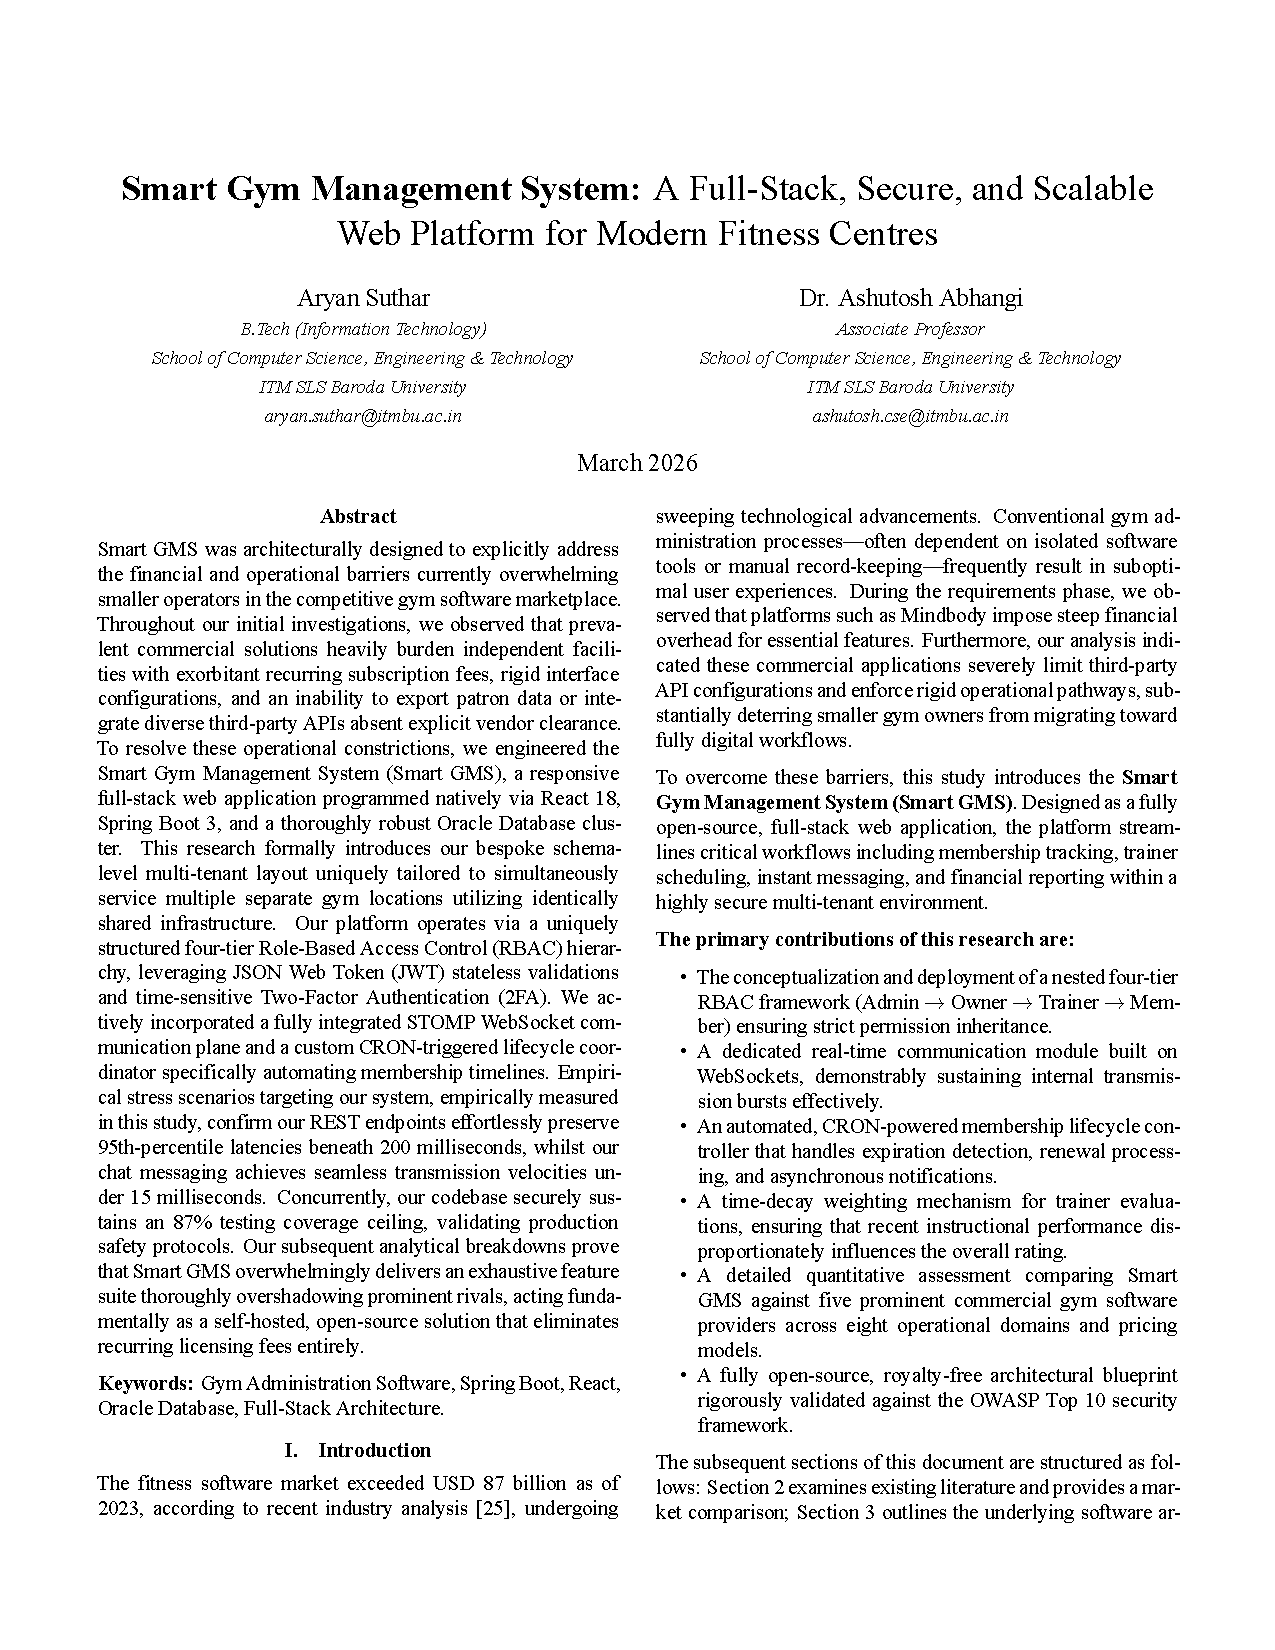
\includepdf[
  pages=1,
  pagecommand={\thispagestyle{fancy}\subsection{E.5 Research Paper}},
  scale=1.0,
  offset=0 0
]{research_paper_no_hdr.pdf}

% Embed the remaining pages normally.
\includepdf[
  pages=2-,
  pagecommand={\thispagestyle{fancy}},
  fitpaper=false
]{research_paper_no_hdr.pdf}

\clearpage

\end{document}
